\documentclass{projetofinal-dcc}

%%%%%%%%%%%%%%%%%%%%%%%%%%%%%%%%%%%%%%%%%%%%%%%%%%%%%%%%%%%%
%P A C O T E S
%%%%%%%%%%%%%%%%%%%%%%%%%%%%%%%%%%%%%%%%%%%%%%%%%%%%%%%%%%%%
% Adicione aqui seus pacotes
\usepackage{todonotes}



%%%%%%%%%%%%%%%%%%%%%%%%%%%%%%%%%%%%%%%%%%%%%%%%%%%%%%%%%%%%
%I N I C I O  D O  D O C U M E N T O
%%%%%%%%%%%%%%%%%%%%%%%%%%%%%%%%%%%%%%%%%%%%%%%%%%%%%%%%%%%%
\begin{document}

% título da tese é obrigatório
\title{Análise e Fomento ao Uso do Laboratório de Informática na Escola: Um Estudo de Caso}

% autor é obrigatório; máximo de 3 autores
\author{Bruno Ricardo Behnken Costa}{Em primeiro lugar e acima de tudo, agradeço a Deus por permitir a realização deste trabalho, e ao meu anjo da guarda, que \textbf{sempre} esteve ao meu lado, principalmente nos momentos mais difíceis.

Agradeço à minha avó Nelly pela incansável dedicação e pelos inigualáveis esforços para me dar suporte e zelar por mim, tolerando com paciência e resignação os momentos em que estive ausente ou estressado por estar assoberbado de afazeres.

À minha mãe, Cláudia, pelo amor e carinho dispensados a mim, por todo o apoio incondicional, pela enorme torcida pelo meu sucesso e por todas as orações e promessas que fez por mim.

À minha tia e madrinha, Nelise, pelos conselhos e pelo interesse na minha vida acadêmica e no meu futuro; e ao meu tio, Ricardo, pelo suporte acadêmico e por estar sempre disponível.

À Profª. Juliana, por me motivar em todos os momentos, por orientar a minha iniciação científica e por me convidar para o Inclusive, projeto precursor deste trabalho. À Profª. Carla, pela orientação sincera e descontraída, presente mesmo em meio a tantos afazeres, com reuniões "no encaixe". Ao Prof. Collier, pela impecável orientação acadêmica. Ao Prof. Gabriel, pela monitoria na disciplina de Arquitetura de Computadores.

Ao Colégio de Aplicação da UFRJ, que acolheu o projeto e permitiu o desenvolvimento deste trabalho.

À minha família, de um modo geral, por todo o apoio e compreensão. A todos os meus amigos na faculdade, que fizeram trabalhos comigo e estiveram ao meu lado nos momentos tristes e felizes.}
\author{Filipe José Teixeira de Oliveira}{Primeiramente, agradeço à minha famíĺia a quem tanto amo, pela paciência e compreensão que forneceram à mim ao longo do curso de Ciência da Computação. Em especial, agradeço à minha mãe, Juciara Teixeira, e ao meu pai, Antonio Oliveira, por oferecerem todo o amor e apoio incondicional para meu sucesso.

Agradeço à Profª. Carla por ter despertado em mim o interesse pela área de Informática Aplicada ao Ensino e pela incrível orientação neste trabalho.

Agradeço ao grande amigo e professor Luiz Oliveira por todo auxílio acadêmico, mentoria e desenvolvimento profissional ao longo de anos.

Agradeço também à Letícia Fassarella, que acompanhou de perto toda a minha trajetória na UFRJ, me acolhendo com paciência, amor e motivação para continuar. Sem dúvidas, você foi fundamental para mim.

À minha grande amiga Pâmela Mizurini, que me auxiliou a refletir melhor sobre diversos aspectos da vida, principalmente o acadêmico.

Ao Colégio de Aplicação da UFRJ, que acomodou o projeto e permitiu o desenvolvimento deste trabalho.}

% orientador é obrigatório
\advisor[Profª.]{Carla Amor Divino Moreira Delgado,~D.Sc.}{}

% co-orientador é opcional
%\coadvisor[Prof.]{Nome do co-orientador,~M.Sc.}{}

% máximo de 3 integrantes da banca (orientador e co-orientador já são adicionados automaticamente)
\banca[Profª.]{Juliana Vianna Valério,~D.Sc.}{}
\banca[Profª.]{Ana Luísa de Cerqueira Leite Duboc,~D.Sc.}{}
%\banca[Prof.]{Nome do participante banca 3,~Ph.D.}{COPPE~-~UFRJ}

\location{Rio~de~Janeiro}{RJ}{Brasil}

% mês e ano de defesa
\date{Março}{2019}
\maketitle

\startdocument

%%%%%%%%%%%%%%%%%%%%%%%%%%%%%%%%%%%%%%%%%%%%%%%%%%%%%%%%%%%%
% D E D I C A T O R I A (opcional)
%%%%%%%%%%%%%%%%%%%%%%%%%%%%%%%%%%%%%%%%%%%%%%%%%%%%%%%%%%%% 
\makededicationpage

%%%%%%%%%%%%%%%%%%%%%%%%%%%%%%%%%%%%%%%%%%%%%%%%%%%%%%%%%%%%
% A G R A D E C I M E N T O S
%%%%%%%%%%%%%%%%%%%%%%%%%%%%%%%%%%%%%%%%%%%%%%%%%%%%%%%%%%%% 
\makethankspage

%%%%%%%%%%%%%%%%%%%%%%%%%%%%%%%%%%%%%%%%%%%%%%%%%%%%%%%%%%%%
% E P I G R A F E (opcional)
%%%%%%%%%%%%%%%%%%%%%%%%%%%%%%%%%%%%%%%%%%%%%%%%%%%%%%%%%%%% 
\makeepigraphpage

%%%%%%%%%%%%%%%%%%%%%%%%%%%%%%%%%%%%%%%%%%%%%%%%%%%%%%%%%%%%
% R E S U M O
%%%%%%%%%%%%%%%%%%%%%%%%%%%%%%%%%%%%%%%%%%%%%%%%%%%%%%%%%%%%
\begin{abstract}{
  A Informática Educativa é uma área reconhecidamente necessária para a modernização da escola e de seus métodos, e o computador pode atuar como catalisador do processo de ensino e aprendizado, se bem utilizado. Entretanto, a simples presença de um laboratório com os seus computadores não garante uma implementação eficiente da Informática Educativa. É necessário que os docentes elaborem propostas pedagógicas para o laboratório, que o laboratório possua o seu próprio projeto pedagógico, que a sala seja adequada, que seja realizada manutenção nos computadores e nos demais equipamentos, que seja oferecida formação continuada aos atores envolvidos na prática da Informática Educativa; dentre outras imposições.
Nesse contexto, este trabalho se propõe a analisar o uso e a gestão do Laboratório de Informática Educativa do CAp-UFRJ, bem como a fomentar uma melhor implementação da Informática Educativa neste colégio, auxiliando na elaboração e execução de uma proposta pedagógica utilizando o laboratório; além de identificar, discutir e propor soluções para problemas existentes.
}
\bigskip
% Palavras-chave separadas por ponto
\palavraschave{Informática Educativa. Laboratório. CAp-UFRJ. Proposta Pedagógica}
\end{abstract}

%%%%%%%%%%%%%%%%%%%%%%%%%%%%%%%%%%%%%%%%%%%%%%%%%%%%%%%%%%%%
% A B S T R A C T
%%%%%%%%%%%%%%%%%%%%%%%%%%%%%%%%%%%%%%%%%%%%%%%%%%%%%%%%%%%%
\begin{englishabstract}{
  The Educational Informatics is an area recognized as necessary for the modernization of the school and its methods, and the computer can act as a catalyst for the teaching and learning process, if well used. However, the mere presence of a laboratory with its computers does not guarantee an efficient implementation of Educational Informatics. It is necessary for teachers to prepare pedagogical proposals for the laboratory, for the laboratory to have its own pedagogical project, for the room to be adequate, for maintenance of computers and other equipment, and for the continuous training of the actors involved in the practice of Educational Informatics; among other impositions.
In this context, this paper proposes to analyze the use and management of the Educational Computer Laboratory of CAp-UFRJ, as well as to promote a better implementation of Educational Informatics in this school, assisting in the elaboration and execution of a class using the laboratory in partnership with a mathematics teacher; besides identifying, discussing and proposing solutions to existing problems.
}
\bigskip
% Palavras-chave separadas por ponto
\keywords{Educational Informatics. Laboratory. CAp-UFRJ. Pedagogical Proposal}
\end{englishabstract}

%%%%%%%%%%%%%%%%%%%%%%%%%%%%%%%%%%%%%%%%%%%%%%%%%%%%%%%%%%%%
% L I S T A S
%%%%%%%%%%%%%%%%%%%%%%%%%%%%%%%%%%%%%%%%%%%%%%%%%%%%%%%%%%%%
% Figuras (opcional)
\makefigurespage

% Tabelas (opcional)
% \maketablespage

% Algoritmos
%\makelistingspage

% Abreviaturas (devem estar em ordem alfabética)
\makeabrevpage{\item [CAp] Colégio de Aplicação da Universidade Federal do Rio de Janeiro
\item [CAp-UFRJ] Colégio de Aplicação da Universidade Federal do Rio de Janeiro
\item [CCS] Centro de Ciências da Saúde
\item [CFCH] Centro de Filosofia e Ciências Humanas
\item [DAE] Direção Adjunta de Ensino
\item [DALPE] Direção Adjunta de Licenciatura, Pesquisa e Extensão
\item [DG] Direção Geral
\item [IE] Informática Educativa
\item [LIE] Laboratório de Informática Educativa
\item [LIG] Laboratório de Informática de Graduação
\item [LoL] \textit{League of Legends}
\item [NCE] Núcleo de Computação Eletrônica
\item [NTIC] Novas Tecnologias de Informação e Comunicação
\item [NUTES] Núcleo de Tecnologia, Educação e Saúde
\item [PUC-RJ] Pontifícia Universidade Católica do Rio de Janeiro
\item [TIC/UFRJ] Superintendência de Tecnologia da Informação e Comunicação da Universidade Federal do Rio de Janeiro
\item [TV] Televisão
\item [UFRJ] Universidade Federal do Rio de Janeiro
}

% Símbolos (devem estar em ordem alfabética)
% \makesymbolspage{\item [I$^2$C] Inter-Integrated Circuit
\item [SRAM] Static Random-Access Memory
\item [EEPROM]  Electrically Erasable Programmable Read-Only Memory
\item [LED] Light-Emitting Diode
\item [MLP] Modulação por Largura de Pulso
\item [PWM] Pulse-Width Modulation
\item [PID] Proportional–Integral–Derivative
\item [RAM] Random-Access Memory
\item [API] Application Programming Interface
\item [GPL] GNU General Public License
\item [GNU] GNU's Not Unix
\item [iid] Independente e identicamente distribuídas}

% Sumário 
\maketocpage

%%%%%%%%%%%%%%%%%%%%%%%%%%%%%%%%%%%%%%%%%%%%%%%%%%%%%%%%%%%%
% C O N T E Ú D O
%%%%%%%%%%%%%%%%%%%%%%%%%%%%%%%%%%%%%%%%%%%%%%%%%%%%%%%%%%%%
\startcontent
\chapter{Introdução}\label{chp:LABEL_CHP_INT}

O laboratório de informática do CAp-UFRJ (Colégio de Aplicação da Universidade Federal do Rio de Janeiro) foi reaberto no ano de 2016, e desde então o seu uso livre é permitido aos estudantes do Ensino Médio e Fundamental II, para que estes utilizem os equipamentos para pesquisas, realização de trabalhos, uso de redes sociais e jogos.

Entretanto, percebeu-se que o uso livre do laboratório é majoritariamente para jogos de entretenimento. Considerando que o uso do computador é, por si só, positivo, canalizar tal uso para atividades com foco educacional pode favorecer a melhor compreensão, por parte do aluno, do potencial do computador para o estudo e para a construção do conhecimento (de acordo com a faixa etária) e, consequentemente, gerar melhor usufruto do equipamento disponível no laboratório.

\section{A Parceria com a Profª. Cassandra}\label{chp:LABEL_CHP_INT_SEC_PARC}

Para colocar em prática este objetivo, buscamos a parceria de um docente do CAp, e, em uma reunião do setor multidisciplinar, que cuida das séries iniciais do ensino fundamental, conhecemos a Profª. Cassandra Marina da Silveira Pontes da Silva, que, no ano de 2018, estava responsável por ministrar a disciplina de matemática para uma turma do 5º (quinto) ano fundamental.

Ao conhecer a Profª. Cassandra, apresentamos a ela nossos anseios de canalizar o uso do laboratório para atividades com foco educacional, e perguntamos se haveria possibilidade de estabelecermos uma parceria, de modo que ela ministrasse uma aula no laboratório aos seus alunos contando com o nosso auxílio, ao que ela aquiesceu, visivelmente empolgada com a perspectiva.

Acordamos então que nesta aula seria abordado o conteúdo de frações com uma turma de alunos do 5º (quinto) ano fundamental utilizando o software educacional \textit{JFraction Lab}\footnote{\textit{Software} educacional desenvolvido com a tecnologia \textit{Java} que trabalha o conteúdo de frações utilizando recursos visuais, como gráficos, e possibilitando ao aluno praticar com exercícios de operações básicas, como soma e simplificação de frações.}, e que nós auxiliaríamos a professora nesta aula.

\section{Objeto da Pesquisa}\label{chp:LABEL_CHP_INT_SEC_OBJ}

Este trabalho tem a proposta de abordar, com crianças do 5º (quinto) ano fundamental, alunas do CAp-UFRJ, o conteúdo de frações utilizando os computadores do LIE (Laboratório de Informática Educativa), em parceria com uma docente de Matemática.

\subsection{Objetivo Geral}\label{chp:LABEL_CHP_INT_SEC_OBJ_SUBSEC_OBJ_GER}

Oferecer opções diversificadas de uso do computador para crianças do 5º (quinto) ano fundamental, de forma que elas ampliem seu entendimento sobre o potencial dessa ferramenta e construam conhecimento tanto acerca do conteúdo de frações quanto acerca da informática de um modo geral, respeitadas as limitações da faixa etária.

\subsection{Objetivos Específicos}\label{chp:LABEL_CHP_INT_SEC_OBJ_SUBSEC_OBJ_ESP}

\begin{itemize}
\item Trabalhar o conteúdo de frações utilizando o computador com alunos do 5º (quinto) ano fundamental em parceria com uma docente de Matemática.

\item Desenvolver estratégias para trabalhar o conteúdo de frações com crianças do 5º (quinto) ano fundamental.

\item Fomentar um projeto de extensão no qual os alunos da área de computação possam auxiliar os docentes do CAp-UFRJ na elaboração de propostas didáticas utilizando o computador, e, assim, fomentar o uso do Laboratório de Informática Educativa entre estes docentes.
\end{itemize}

\section{Metodologia}\label{chp:LABEL_CHP_INT_SEC_MET}

A metodologia de pesquisa será pesquisa-ação, ou seja, será desenvolvida uma estratégia que será aplicada e avaliada, e os resultados tem por objetivo o aumento da compreensão do objeto da pesquisa. Pretende-se diagnosticar a abordagem do conteúdo de frações, bem como a utilização do LIE por parte dos professores, por meio de métodos etnográficos (cujo objetivo é o estudo de pessoas e culturas), observação participante, questionários e entrevistas com gestores, professores, bolsistas e alunos; pesquisando soluções possíveis que atendam a demandas específicas do grupo e da comunidade.

\section{Organização do Trabalho}\label{chp:LABEL_CHP_INT_SEC_ORG}

A organização deste trabalho formata-se em cinco capítulos. O primeiro apresenta a introdução ao tema, a proposta da pesquisa e a organização do trabalho.

O segundo capítulo expõe o referencial teórico que fundamenta a inserção das NTIC (Novas Tecnologias de Informação e Comunicação) na escola, tratando de inclusão digital, da informática educativa, do laboratório de informática educativa e do papel dos professores e dos gestores.

O terceiro capítulo apresenta um resumo das entrevistas que realizamos com diversos atores envolvidos na informática educativa no CAp, e tece considerações a respeito delas.

O quarto capítulo expõe o relato da tentativa que fizemos de ministrar uma aula no laboratório em parceria com uma professora, enumera as dificuldades que enfrentamos e articula considerações sobre o que foi exposto.

O quinto capítulo apresenta a conclusão à qual chegamos, bem como a aceitação dela por parte do CAp; tece considerações finais e apresenta possibilidades de trabalhos futuros.

\chapter{Referencial Teórico}\label{chp:LABEL_CHP_REF_TEO}

Na sociedade contemporânea, é notória a influência que exerce a tecnologia. Se há poucas décadas o computador se introduzia lentamente na rotina dos cidadãos, hoje está presente não apenas nas mesas de trabalho, na forma de \textit{desktops} e \textit{notebooks}, mas também nos bolsos, na forma de celulares, e, mais recentemente, em várias partes do corpo, na forma de relógios, óculos e pulseiras inteligentes, dentre outros \textit{wearables}.

Diante de um cenário de constante mudança, é natural que as instituições mais tradicionais tenham dificuldades em acompanhar a rápida evolução das NTIC. Neste contexto, a situação da escola é delicada pois ela lida diretamente com jovens que muitas vezes possuem amplo acesso a tecnologias de ponta logo nos primeiros anos de vida, e demonstram ser donos de uma perícia que está muito além das habilidades de seus professores.

Por outro lado, a escola também recebe jovens que possuem pouco ou nenhum acesso à tecnologia, e que não dispõem de conhecimentos básicos acerca dela. Sobre isso, afirma Mattos \cite{art:REF_ART_MATTOS} que, em 2008, apenas 21\% da população brasileira e apenas 26,7\% da população fluminense utilizava a Internet. A desigualdade no acesso à tecnologia, um traço tão marcante da sociedade contemporânea, nunca esteve tão bem representada na sala de aula.

\section{A Importância da Inclusão Digital}\label{sec:LABEL_CHP_REF_TEO_SEC_ID}

Neste contexto, a inclusão digital promovida a partir da escola assume importância fundamental para reduzir a desigualdade social do nosso país. A respeito do Proinfo, programa de inclusão digital do Governo Federal, afirmam Carvalho e Monteiro \cite{art:REF_ART_CARVALHO_MONTEIRO} que "a preocupação oficial no Brasil em relação à introdução da informática nas redes de ensino, bem como sobre seu acesso, usos e possibilidades na escola alia-se a discussões sobre a necessidade de equalizar as oportunidades de inclusão digital para grupos sociais excluídos".

A inclusão digital, que antes era considerada ferramenta de redução da desigualdade social, hoje se configura como ferramenta essencial para o não aprofundamento desta desigualdade, uma vez que "na realidade brasileira, as pessoas participantes de diversos contextos sociais estão tendo um crescente acesso a computadores enquanto ferramenta de trabalho" \cite{art:REF_ART_CARVALHO_MONTEIRO}.

A habilidade no uso das NTIC vem sendo colocada pelos empregadores como exigência mínima para a contratação para as suas vagas de emprego, ainda que em cargos que exijam pouca formação acadêmica e que possuam baixa remuneração. Se os grupos sociais excluídos permanecerem sem acesso às NTIC, estes terão cada vez menos competitividade no mercado de trabalho, o que contribuirá para aprofundar ainda mais as desigualdades sociais.

\section{A Importância da Informática Educativa}\label{sec:LABEL_CHP_REF_TEO_SEC_IE}

A inclusão digital, apesar de importante, não deve ser o único aspecto da informática nas escolas, que têm como missão a realização dos objetivos pedagógicos e educacionais. O computador é uma ferramenta poderosa, que em muito pode contribuir para a pedagogia. "Entretanto, constata-se em algumas realidades escolares, a ausência de uma visão mais ampliada da utilização do computador enquanto um mediador na construção de conhecimentos" \cite{art:REF_ART_CARVALHO_MONTEIRO}.

Neste contexto, afirma Dutra \cite{art:REF_DISS_DUTRA} que "o uso das NTIC no ensino constitui em um dos aspectos considerados importantes para a modernização da escola e da educação. A essas tecnologias é depositada a possibilidade de transformar o ensino, de dar mais autonomia ao aluno, alterando a relação professor-aluno e aponta para mudanças na estrutura e funcionamento da escola". Entretanto, "enquanto a sociedade muda e experimenta desafios mais complexos, a educação formal continua, de maneira geral, organizada de modo previsível, repetitivo, burocrático, pouco atraente" \cite{art:REF_LIVRO_MORAN}.

Fica evidente a necessidade de a escola introduzir na sua rotina as NTIC, uma vez que elas podem ser um agente catalisador do processo de aprendizado, contribuindo efetivamente para este, além de atuarem como fator motivacional para os alunos, que se sentem felizes e demonstram maior engajamento ao projeto pedagógico quando este envolve o uso da tecnologia.

Apesar de concordar com tais afirmações, Odorico \cite{art:REF_ART_ODORICO} realiza uma ressalva: "Atualmente, a informática cresce em uso e relevância em todo o mundo possibilitando trazer inúmeros desenvolvimentos de atividades diferenciadas para a sala de aula. As atividades utilizando recursos computacionais podem contribuir de forma efetiva para o processo ensino aprendizagem, desde que haja contribuição dos programas governamentais, apoio técnico, capacitação e planejamento dos educadores".

Eis que surge um dos desafios da Informática Educativa (IE): como criar e executar, em uma escola, um projeto pedagógico que utilize de maneira significativa as NTIC e atenda tanto a alunos que possuem alto grau de acesso à tecnologia (e apresentam admiráveis habilidades com ela) quanto a alunos que possuem pouco ou nenhum grau de acesso? Um ponto importante e ainda mais desafiador: como elaborá-lo sem introduzir segmentações ou discriminações entre esses grupos de alunos?

\section{O Laboratório de Informática Educativa}\label{sec:LABEL_CHP_REF_TEO_SEC_LIE}

O primeiro passo, evidentemente, surge de modo natural: é necessário que a escola possua equipamentos disponibilizados em uma sala adequada para que seja possível executar este projeto pedagógico. Em outras palavras, é necessário que a escola possua um Laboratório de Informática Educativa (LIE).

Entretanto, apenas a construção de um LIE não é o suficiente para uma implementação eficiente da IE. Sobre isso, afirma Odorico \cite{art:REF_ART_ODORICO} que "muitas instituições que inseriram Laboratórios de Informática em seu meio não conseguiram realizar as modificações esperadas, sendo estes espaços considerados na maioria dos casos enfeites".

O que se observa é que existe a ideia, construída pela mídia e utilizada como \textit{marketing} por algumas instituições de ensino, "de que com laboratórios instalados nas escolas teremos automaticamente cursos melhores e resolvidos os nossos centenários problemas educacionais (...). Como em outras épocas, há uma expectativa de que as novas tecnologias nos trarão soluções rápidas para mudar a educação" \cite{art:REF_LIVRO_MORAN}.

É importante ter em mente que a tecnologia, por si, não modifica projetos pedagógicos e não oferece melhores resultados acadêmicos. É necessário pensá-la como recurso didático, como ferramenta de ensino, e elaborar projetos pedagógicos levando em consideração as possibilidades e limitações da tecnologia, de modo que se possa aproveitá-la em todo o seu potencial. Conforme colocado por Moran \textit{et al} em seu livro \cite{art:REF_LIVRO_MORAN}, "não são os recursos que definem a aprendizagem, são as pessoas, o projeto pedagógico, as interações, a gestão".

É necessário que o Laboratório de Informática Educativa seja considerado como um recurso didático da escola, e não apenas como uma sala de informática, onde os alunos (nem sempre) podem entrar. É necessário que este recurso seja considerado no momento da elaboração dos projetos pedagógicos, seja da escola como um todo, onde o laboratório pode atuar como ferramenta multidisciplinar, unificando objetivos de componentes curriculares diferentes; seja das disciplinas isoladamente, onde o professor pode (e deve) utilizar o laboratório como catalisador do processo de aprendizado, para chegar de maneira mais rápida e mais efetiva aos seus objetivos pedagógicos.

Ao tomarmos consciência de que este processo não é realizado nas escolas, é natural que busquemos as razões que levam a isto. A literatura aponta que as mais relevantes razões pelas quais a IE não é bem implementada mesmo com a presença do LIE são a resistência inicial dos professores da escola e dos gestores.

\subsection{O papel dos professores}\label{sec:LABEL_CHP_REF_TEO_SEC_RES_PROF}

A respeito da resistência inicial dos professores, relata Chagas \cite{art:REF_ART_CHAGAS} em sua investigação que "era transparente nos docentes, a resistência em querer integrar o LIE em suas atividades pedagógicas, pois já têm internalizado procedimentos didáticos-práticos sem o uso do computador. Vários são os termos usados pelos docentes em seus discursos quanto ao conhecimento dos recursos tecnológicos, tais como 'sou totalmente leigo em informática' ou 'sou leigobyte' ou 'analfabyte' ou 'informática é muito difícil'. Afirmações como estas vêm para reforçar a barreira inicial criada pelo professor diante do computador".

Entretanto, é necessário ter em mente que "o professor tem a responsabilidade de preparar o aluno para se tornar um cidadão ativo dentro da sociedade, apto a questionar, debater e romper paradigmas" \cite{art:REF_ART_OLIVEIRA}.

No contexto da sociedade contemporânea, onde a tecnologia exerce crescente influência em diversos setores, é razoável considerar que um cidadão ativo é um cidadão que sabe utilizar as NTIC, uma vez que o domínio delas é necessário para realizar atividades de cidadania, como declarar o Imposto de Renda. % [este assunto já foi abordado acima] É notório também que muitas empresas, não necessariamente grandes, têm inserido o domínio das NTIC nos requisitos de suas vagas de emprego, mesmo em funções que não necessitam de grande formação acadêmica, como caixa de supermercado ou secretário.

No âmbito tecnológico-escolar, o papel do professor é, portanto, preparar seus alunos para a utilização das tecnologias, familiarizando-os com elas e dando subsídios para que estes alunos, no futuro, sejam capazes de aprender por si mesmos a utilizá-las conforme sentirem necessidade.

Apesar de muitos alunos apresentarem pouca ou nenhuma familiaridade com a tecnologia, outros apresentam habilidades que em muito superam a de seus professores. Neste contexto, afirma Odorico \cite{art:REF_ART_ODORICO} que "muitos professores se sentem inseguros quando trabalham com seus alunos no laboratório de informática, pois sabem que estes dominam as máquinas e as ferramentas mais do que eles".

Se a barreira inicial criada pelo professor diante do computador tem como cerne a falta de habilidade deste com as tecnologias e há alunos que as dominam, então, tomando inspiração em Cora Coralina, que declarou que "feliz aquele que transfere o que sabe e aprende o que ensina", cria-se a oportunidade perfeita para que o professor aumente seus conhecimentos de tecnologia aprendendo com os próprios alunos.

Observa-se, portanto, que a principal dificuldade a ser transposta, da parte dos professores, para que eles cumpram com o seu papel é a resistência inicial que possuem.

\subsubsection{O docente do LIE}\label{sec:LABEL_CHP_REF_TEO_SEC_DOC_LIE}

Para amenizar este problema, é fundamental que esteja presente um ator conhecido como "docente do LIE". Este professor possui formação tanto técnica quanto pedagógica, e está capacitado para auxiliar os demais atores (gestores e outros professores) na elaboração e execução de atividades pedagógicas no contexto da Informática Educativa.

A importância da presença do docente do LIE para a implementação eficiente da IE é reforçada por Chagas \cite{art:REF_ART_CHAGAS}: "O desconhecimento técnico mínimo necessário para o uso das novas ferramentas de trabalho, dos softwares educativos, da Internet, de atividades no computador, são pontos fortes (sic) para a não implementação da IE (...). Neste momento, o apoio específico do professor do laboratório se torna indispensável para que se atinja as sonhadas mudanças da IE".

A despeito de tal importância, muitas vezes o docente do LIE não está presente nas escolas. Odorico \cite{art:REF_ART_ODORICO}, ao investigar sobre os laboratórios de duas escolas da rede estadual de ensino de Minas Gerais, constatou que "um fator que pesa muito na utilização dos laboratórios é a presença na escola de um profissional da área de informática, já que muitos professores sentem-se inseguros e apresentam dificuldades para utilizar o computador. Entretanto nenhuma das instituições analisadas possui tal profissional para auxiliar os professores nas matérias específicas".

\subsection{O papel dos gestores}\label{sec:LABEL_CHP_REF_TEO_SEC_RES_GEST}

É notório que os gestores das escolas possuem muitos encargos, que oneram seu trabalho e o tornam desgastante e burocrático. Sobre isso, afirma Groll \cite{art:REF_TCC_GROLL} que "a gestão escolar se confunde, frequentemente, com administração, e não raro com Administração Científica, onde a burocracia impera. Mas o gestor escolar tem, além das tarefas administrativas e burocráticas, seu papel de professor".

Por conta dos encargos das funções de gestão, por vezes os gestores não se mostram interessados em trabalhar melhor o LIE no contexto pedagógico, pois os diversos problemas estruturais se tornarão novos encargos nas suas funções. Entretanto, no contexto do seu papel de professor, "é necessário que os dirigentes escolares atentem para o significado do trabalho de informatização como meio para a realização dos objetivos educacionais de natureza pedagógica, razão última da existência da escola" \cite{art:REF_TCC_GROLL}.

O papel do gestor no processo de implementação da IE na escola é explicitado por Groll \cite{art:REF_TCC_GROLL}: "os gestores, enquanto líderes, devem ser os encaminhadores rumo à tomada de consciência de toda comunidade escolar sobre a nova realidade que vivenciamos e que, portanto, a escola deve ser um ambiente aberto, democrático, flexível e naturalmente adequado para a promoção da inclusão digital e favorecer (sic) a criatividade e a inovação mediante o diálogo entre os vários componentes da comunidade".

% Chagas relata a respeito de cursos de formação para docentes do LIE na página 4 de seu artigo: "Quanto a sua Formação: Cursos de Especialização em Informática Educativa, era um investimento da PMF/Proinfo, para estes professores. Mas, a própria Prefeitura exigia o cumprimento destes profissionais nas atividades na escola".
% Isso pode ou não ser incluído no texto, neste capítulo ou em outro.
\chapter{Compreendendo o Funcionamento do Laboratório}\label{chp:LABEL_CHP_ENT}

\section{A Opção por Entrevistar os Atores}\label{chp:LABEL_CHP_ENT_SEC_OPC}

Para melhor compreender a dinâmica de funcionamento interno do CAp, como o LIE se insere nesse contexto, como o LIE funciona em termos de organização atualmente, quais projetos são desenvolvidos, como as aulas são ministradas, entre outras informações relevantes; optamos por realizar entrevistas com alguns atores que consideramos como fundamentais para o funcionamento efetivo de um LIE.

No caso do CAp, esses atores são a Direção Geral (DG), como gestora de recursos financeiros e da escola como um todo; a Direção Adjunta de Licenciatura, Pesquisa e Extensão (DALPE), como setor responsável pelos recursos pedagógicos da escola, inclusive pelo laboratório; a Profª. Cassandra, que, ao conhecer nosso trabalho, se interessou pela proposta e aceitou utilizar o laboratório com o nosso suporte; e dois bolsistas, cuja função é permanecer no laboratório e auxiliar as atividades desenvolvidas nele.

A partir das entrevistas foi possível observar a situação atual do CAp, entender a dinâmica de funcionamento do laboratório e tirar algumas conclusões sobre os problemas existentes atualmente. As entrevistas também subsidiaram o trabalho que viria a seguir, de tentativa de utilização pedagógica do LIE.

As seções seguintes trazem as perguntas que foram realizadas a cada ator e as conclusões que foram tiradas a partir das respostas que obtivemos. As transcrições completas de todas as entrevistas encontram-se em anexos.

\section{Entrevista com a Direção Geral}\label{chp:LABEL_CHP_ENT_SEC_DG}

Para a diretora geral do CAp-UFRJ, foram realizadas as seguintes perguntas:
\begin{itemize}
\item Você acha importante, ou ao menos pertinente, o uso do laboratório?
\item O que compete ao gestor no uso do laboratório de informática?
\item Como você, como gestora do CAp, considerando as limitações às quais está sujeita, poderia promover o uso do laboratório?
\item Como um gestor hipotético que disponha de todos os recursos que ele quiser poderia promover o uso do laboratório?
\end{itemize}

A partir da entrevista com a diretora geral foi possível perceber que o CAp é aberto à Informática Educativa e à promoção do laboratório como recurso didático do colégio, e que não oferece resistência à esta promoção; bem como foi possível perceber que as principais limitações são relacionadas ao espaço físico e à ausência do docente do LIE, e que essas limitações são conhecidas pela Direção da escola, que demonstrou inclinação a saná-las.

Foi ainda possível compreender que a gestão do laboratório é dividida entre a DG, responsável pela infra-estrutura, e a DALPE, responsável pela administração e pela parte pedagógica do laboratório.

A transcrição completa desta entrevista encontra-se no anexo A.

\section{Entrevista com a Direção Adjunta de Licenciatura, Pesquisa e Extensão}\label{chp:LABEL_CHP_ENT_SEC_DALPE}

Para a diretora adjunta de licenciatura, pesquisa e extensão do CAp-UFRJ foram realizadas as seguintes perguntas:

\begin{itemize}
\item{Quais são as propostas pedagógicas atuais para o uso do laboratório?}
\item{Você acha que uma proposta pedagógica unificada para todos, como sugestão, seria melhor do que propostas individuais?}
\item{Como é utilizado o laboratório?}
\item{Há quantos bolsistas?}
\item{Qual a viabilidade da realização de um projeto de extensão, por parte dos alunos da UFRJ, no laboratório?}
\end{itemize}

A partir da entrevista com a diretora foi possível perceber que o laboratório é mais utilizado para acolher aulas de professores que levam lá as suas turmas, e que estes ficam responsáveis pela elaboração das propostas pedagógicas, o que implica que não necessariamente a proposta elaborada implementará a Informática Educativa. O laboratório não possui projeto pedagógico próprio, mas há, por parte da DALPE, o interesse de elaborar um.

Foi possível perceber que o LIE possui 5 (cinco) bolsistas associados a ele, que o ocupam de 8h às 17h, de segunda à sexta-feira. Os alunos a partir do 6º (sexto) ano fundamental possuem livre acesso ao laboratório, e não há restrições quanto ao uso dos computadores, exceto por um jogo, que teve seu acesso bloqueado por estar causando problemas à ordem. Os bolsistas monitoram as atividade dos alunos no laboratório e auxiliam os professores quando estes ministram suas aulas no LIE.

A diretora relatou que a sala é inadequada, pois é pequena e possui uma pilastra no meio, o que desencoraja o uso do laboratório pelos professores; frisou que não há funcionário responsável pela parte de tecnologia no CAp, e que não há docente no LIE; e mostrou-se aberta à realização de um projeto de extensão no laboratório.

A transcrição completa desta entrevista encontra-se no anexo B.

\section{Entrevista com a Professora Cassandra}\label{chp:LABEL_CHP_ENT_SEC_CASS}

A entrevista com a Professora Cassandra, que dá aulas de matemática para o Fundamental I, foi composta de duas etapas. Na primeira etapa foram feitas as perguntas discriminadas a seguir, e na segunda foi apresentado o software \textit{JFraction Lab} para que ela avaliasse a pertinência de um plano de aula utilizando-o. 

Na primeira etapa foram realizadas as seguintes perguntas:

\begin{itemize}
\item{Você utiliza, ou já utilizou, o laboratório de informática do CAp?}
\item{Por que você não utiliza o laboratório de informática? Gostaria de utilizá-lo? Quais motivações te levariam a sair da sala de aula e levar os alunos ao laboratório?}
\item{Você acha que o uso do laboratório pode ajudá-la a atingir os objetivos da sua disciplina?}
\item{Você vislumbra algum objetivo pedagógico além dos objetivos da sua disciplina para o qual o uso do laboratório possa contribuir?}
\item{Você estaria disposta a nos ajudar a construir uma proposta didática para o uso do laboratório na sua disciplina?}
\item{Se nós elaborarmos uma proposta pedagógica multidisciplinar envolvendo a sua disciplina, você aceitaria participar?}
\item{O que podemos elaborar como proposta pedagógica para o laboratório dentro da sua disciplina ainda para esse ano?}
\end{itemize}

A partir das respostas dadas a estas perguntas, foi possível concluir que a Profª. Cassandra nunca utilizou o laboratório porque nunca parou para planejar uma aula nele, mas que esta vontade está presente, pois ela se sente atraída pela parte gráfica, com representações geométricas e visualizações, utilizando, por exemplo, o \textit{Google Maps}, software que ela vislumbra sendo utilizado de modo multidisciplinar.

Na segunda parte da entrevista, a Profª. Cassandra relatou que estava, naquela época, trabalhando o conteúdo de frações com a sua turma de 5º (quinto) ano, e que seria oportuno utilizar um software que representasse as frações em gráficos como o de pizza, e permitisse que eles treinassem operações básicas, como simplificações. 

Foi apresentado então o software \textit{JFraction Lab}\footnote{\textit{Software} educacional desenvolvido com a tecnologia \textit{Java} que trabalha o conteúdo de frações utilizando recursos visuais, como gráficos, e possibilitando ao aluno praticar com exercícios de operações básicas, como soma e simplificação de frações.}, que atende aos requisitos colocados. A professora se interessou pelo software e se comprometeu a elaborar um plano de aula no laboratório envolvendo o uso deste, conosco acompanhando a aula e ajudando-a a ministrá-la.

Na ocasião da entrevista já deixamos marcado o dia e o horário em que a aula seria ministrada, e ficou acordado que chegaríamos cinquenta minutos antes do início da aula para instalar o software nas máquinas do laboratório.

A transcrição completa desta entrevista encontra-se no anexo C.

\section{Entrevista com a bolsista Ingrid}\label{chp:LABEL_CHP_ENT_SEC_ING}

Para a bolsista Ingrid, que trabalha no LIE, foram realizadas as seguintes perguntas:

\begin{itemize}
\item{Qual o seu curso na UFRJ? Há quanto tempo você está trabalhando como bolsista do laboratório? Quais são os seus horários aqui?}
\item{Você acha que muitas crianças vêm ao laboratório? Quantas, mais ou menos?}
\item{Em geral, o que elas fazem no computador?}
\item{Como funciona o processo de supervisão das crianças no laboratório?}
\item{Você ajuda os professores que trazem seus alunos para realizar tarefas no laboratório?}
\item{Quais as principais demandas que surgem no dia a dia?}
\end{itemize}

A partir da entrevista com a bolsista foi possível perceber que de 20 (vinte) a 25 (vinte e cinco) alunos visitam o LIE todas as tardes. As principais atividades deles no laboratório são fazer trabalhos e assistir vídeos no \textit{YouTube}, entretanto a maioria dos vídeos possui áudio, e o LIE possui apenas um fone de ouvido para disponibilizar aos alunos. Além disso, alguns alunos gostariam de acessar jogos \textit{on-line}, mas esse acesso foi bloqueado.

Por conta do uso indevido do laboratório, foram colados avisos de relacionamento com o espaço nas paredes. Foi relatado que esses avisos auxiliam na supervisão dos alunos no laboratório.

Foi possível saber também que os professores realizam o agendamento de suas aulas no laboratório por meio de uma planilha que fica disponível \textit{on-line} para todos os professores, e que as principais demandas que eles apresentam aos bolsistas são de ordem técnica -- os planos de aula, bem como a sua execução, são realizados sem a ajuda dos bolsistas.

A transcrição completa desta entrevista encontra-se no anexo D.

\section{Entrevista com o bolsista Pedro}\label{chp:LABEL_CHP_ENT_SEC_PED}

Para o bolsista Pedro, que trabalha no LIE, foram realizadas as seguintes perguntas:

\begin{itemize}
\item{Qual o seu curso na UFRJ? Há quanto tempo você está trabalhando como bolsista do laboratório?}
\item{Você acha que muitas crianças vêm ao laboratório? Quantas, mais ou menos?}
\item{Em geral, o que os alunos fazem no computador?}
\item{Como funciona o processo de supervisão das crianças no laboratório?}
\item{Você ajuda os professores que trazem seus alunos para realizar tarefas no laboratório?}
\item{Quais as principais demandas que surgem no dia a dia?}
\item{Você acha que o laboratório atrairia mais os alunos se oferecesse mais coisas a eles?}
\item{Quais são os principais problemas que você identifica no laboratório?}
\item{Você está se formando em Educação Física. Como docente deste componente curricular, você usaria o laboratório? Como?}
\item{Ouvimos da bolsista Ingrid que certa vez tentaram instalar o \textit{LoL}\footnote{\textit{League of Legends}. Jogo eletrônico da categoria MOBA (\textit{Multiplayer Online Battle Arena}) desenvolvido pela empresa \textit{Riot Games}. É muito popular entre os jovens brasileiros.} em um dos computadores. Esse é um jogo muito famoso, o maior expoente do \textit{e-sports}, que é uma área que se integra com a Educação Física, sua área de formação. Considerando que a procura por jogos aqui no laboratório é grande, você o utilizaria para fazer algo na área de \textit{e-sports} com os alunos do CAp?}
\end{itemize}

A partir da entrevista com o bolsista foi possível perceber que o número de alunos que frequenta o laboratório varia durante o ano, e é mais expressivo no início dos períodos letivos, e menos expressivo no final. Como a entrevista foi realizada em novembro, naquela época a frequência média de alunos era de 10 (dez) por dia.

Foi possível perceber também que a maior demanda dos alunos é por vídeos no \textit{YouTube} e jogos \textit{on-line}, o que condiz com o que foi relatado pela bolsista Ingrid. Há ainda uma grande demanda por impressões de trabalhos, da parte dos alunos, e por impressões de provas, da parte dos professores. Os professores que dão aula no laboratório por vezes apresentam também a demanda de instalação de software e de testes de vídeos a serem exibidos, a fim de se assegurarem de que tudo funcionará corretamente no momento da aula.

Foi relatado ainda que a função do bolsista é de zelar pelo uso do laboratório e que a supervisão dos alunos consiste em observá-los e intervir caso estejam fazendo uso inadequado do espaço.

Assim como relatado pela bolsista Ingrid, o bolsista Pedro também informou que os professores realizam o agendamento da aula utilizando uma planilha \textit{on-line}, entretanto, foi dito que poucos professores utilizam o laboratório, uma estimativa de quatro ou cinco, e que são sempre os mesmos. Estes muitas vezes não usam os recursos computacionais do laboratório, apenas a televisão como recurso multimídia. Neste contexto, o bolsista informou que sente falta de um \textit{workshop} voltado para o uso dos recursos computacionais do laboratório, pois a televisão é o recurso mais utilizado pelos professores.

Quanto aos problemas, conforme relatado por outros atores, o bolsista informou que a pilastra no meio da sala acaba sendo problemática, pois o professor não possui uma visão completa da sala. O laboratório é pequeno, e com turmas grandes se torna necessário que os alunos dividam os computadores, e isso, por vezes, gera alguns atritos entre eles. O ar-condicionado que pinga dentro do laboratório é o principal problema atualmente.

Além disso, foi colocado como um problema a manutenção do laboratório ficar a cargo dos bolsistas, principalmente porque há equipamentos que eles não sabem consertar, como a impressora, que havia quebrado há algumas semanas e permanecia assim, aguardando manutenção especializada -- enquanto isso, as demandas por impressão, recorrentes no laboratório, não estavam sendo atendidas.

O bolsista relatou ainda o desejo de utilizar um \textit{kinect} no laboratório, junto com um projetor e um \textit{X-Box}, pois estes equipamentos seriam relevantes para o ensino da Educação Física. Mostrou ainda a vontade de desenvolver uma proposta pedagógica no LIE que utilizasse os \textit{e-sports}, pois os alunos demonstram uma forte aderência a eles.

A transcrição completa desta entrevista encontra-se no anexo E.

\section{O que Percebemos e Concluímos}\label{chp:LABEL_CHP_ENT_OBS_CONC}

As entrevistas que realizamos com os diversos atores ligados ao LIE foram fundamentais para termos uma melhor percepção do \textit{modus operandi} do CAp e do laboratório em si. A partir delas foi possível observar e concluir diversas coisas.

O LIE do CAp não possui o seu próprio docente, ator classificado como indispensável por Chagas \cite{art:REF_ART_CHAGAS}; entretanto, esta função é, até certo ponto, desempenhada por bolsistas da própria UFRJ. Portanto, conclui-se que, apesar da ausência do docente do LIE no laboratório do CAp, a situação não é tão precária quanto a que Odorico \cite{art:REF_ART_ODORICO} encontrou nas escolas que visitou na rede estadual de Minas Gerais, pois estas não possuíam nem mesmo bolsistas ou estagiários.

Entretanto, pudemos perceber que a presença dos bolsistas não é suficiente para fomentar a implementação da Informática Educativa, fato evidenciado nas duas entrevistas realizadas com os gestores (DG e DALPE), que demonstraram desejo de que o laboratório fosse mais utilizado para fins pedagógicos, tanto no contexto de cada disciplina isolada quanto no contexto do colégio como um todo.

Fica evidente que os bolsistas não têm possibilidade de desenvolver projetos na área de IE, ainda que estes queiram fazê-lo, e esta vontade se mostra presente, conforme evidenciado pelo bolsista Pedro no final de sua entrevista. Isto se dá pois os bolsistas não possuem vínculo empregatício com o CAp, e não podem ser responsabilizados por projetos ou por eventuais problemas que venham a acontecer no laboratório.

Por conta da ausência do docente do LIE, os bolsistas acabam também assumindo encargos que não deveriam (e talvez nem poderiam) ser seus, tais como a manutenção de hardware e software das máquinas no laboratório, bem como a responsabilidade de decidir se um software deve ou não ser instalado no computador (encargo evidente no relato da visita que realizamos) ou se um site ou software deve ser acessado ou não pelos alunos.

Neste contexto, identificamos uma contradição nas entrevistas. A Profª. Isabel, gestora da DALPE, relatou que o uso de jogos era liberado no laboratório, com exceção de um jogo específico, entretanto, a bolsista Ingrid relatou que os jogos \textit{on-line} estavam com acesso bloqueado, fato que pôde ser comprovado por nós naquela data. Surgiu então uma dúvida a respeito da sinergia entre os bolsistas e a DALPE.

Apresentamos à Profª. Isabel a informação de que os jogos \textit{on-line} estavam bloqueados e perguntamos se o bloqueio que fora realizado havia sido autorizado, ao que ela redarguiu que apenas um jogo deveria ser bloqueado pelos bolsistas, mas que ela não sabe como funciona o processo de bloqueio a esse jogo, e que há a possibilidade de que a solução técnica encontrada pelos bolsistas para este problema acabe por bloquear também o acesso a outros jogos.

Identificamos, assim, que a falta de preparo técnico dos bolsistas compromete os objetivos estabelecidos pela DALPE, uma vez que há melhores soluções do ponto de vista técnico para o bloqueio do acesso a um jogo; e que a sinergia entre estes dois atores fundamentais não é tão grande quanto desejável, uma vez que não foi informado à DALPE que o procedimento de bloquear todos os jogos \textit{on-line} seria tomado para efetivar o bloqueio a um único jogo.

Outra observação importante é a respeito da nomenclatura do laboratório. A Profª. Isabel se referiu a ele como "LIG", que significa Laboratório de Informática de Graduação, nome que não reflete com exatidão os objetivos pedagógicos do ensino básico. Não temos por objetivo discutir assuntos pouco relevantes, como a nomenclatura adotada; entretanto, este é um indício de que talvez a Informática Educativa não esteja muito bem definida para a gestão do CAp.

No mais, as entrevistas permitiram o conhecimento da dinâmica de funcionamento do laboratório: ele fica aberto aos alunos, que podem entrar e sair livremente se forem do Fundamental II ou do Ensino Médio, e podem usar o computador da maneira que quiserem, respeitadas algumas restrições. Se um professor quiser ministrar uma aula no laboratório, é necessário reservá-lo, e esta reserva é realizada através de uma planilha \textit{on-line} que fica disponível para os professores. O suporte técnico para a aula pode ser solicitado pelo professor e é oferecido pelos bolsistas. Além dos computadores, o laboratório possui um aparelho de televisão.

\chapter{A Tentativa de Aula com a Profª. Cassandra}\label{chp:LABEL_CHP_REL}

\section{Introdução}\label{sec:LABEL_CHP_REL_SEC_INTRO}

No dia 31 de outubro de 2018 Bruno esteve em reunião com a professora Cassandra, na qual foi realizada a entrevista que foi relatada na seção \ref{chp:LABEL_CHP_ENT_SEC_CASS}. Nesta reunião, foi acordado que no dia 14 de novembro o laboratório seria utilizado pela Cassandra em parceria conosco para ministrar uma aula no software \textit{JFractionLab}. Ficou acordado que chegaríamos no CAp às 13h para realizar a instalação do software nas máquinas do laboratório, para que às 13h50min (início do segundo tempo de aula) a Cassandra pudesse levar os alunos ao laboratório e ministrar a aula com o nosso auxílio.

O presente relato visa expor as experiências que vivemos naquele dia e as informações que recolhemos, bem como os problemas que enfrentamos e percebemos. Separamos os problemas em tópicos, e, para cada um deles, formulamos alguns questionamentos, que foram levados à DALPE. Na seção \ref{sec:LABEL_CHP_REL_SEC_PROBS}, ao final deste capítulo, estão discriminados estes tópicos, bem como os questionamentos formulados e as respostas que foram dadas a eles.

\section{Relato do Dia da Aula}\label{sec:LABEL_CHP_REL_SEC_REL}

% \subsection{A Espera}\label{sec:LABEL_CHP_REL_SEC_REL_SUBSEC_ESP}

No dia 14 de novembro, quarta-feira, às 13 horas, chegamos no CAp para realizar a instalação do software nas máquinas, entretanto, a bolsista que estava responsável pelo laboratório naquele horário, que deveria chegar também às 13h, não estava presente. Fomos à DALPE e lá nos informaram que a única saída seria aguardar, pois não era possível entregar a chave do laboratório a uma pessoa que não possuísse vínculo com o CAp. Aguardamos, então que a bolsista chegasse, o que só se concretizou às 13h45min, cinco minutos antes do segundo tempo, horário combinado com a Cassandra para trazer os alunos ao laboratório.

Ao longo do tempo de espera, estivemos sentados em frente à porta do laboratório, e pudemos constatar que diversos alunos procuraram o LIE para utilizá-lo, mas o encontraram vazio, com a porta trancada.

% \subsection{Problemas Estruturais Encontrados}\label{sec:LABEL_CHP_REL_SEC_REL_SUBSEC_PROB}

Na ocasião da chegada da bolsista, o laboratório foi aberto por ela e constatou-se que estava trancada a porta interna do laboratório, que dá acesso à área onde fica o computador utilizado pelos bolsistas e outros materiais relevantes. A bolsista responsável naquele momento disse que apenas um outro bolsista tinha a chave, mas que ele já havia ido embora. Relatou que a DALPE não possuía cópia da chave, e que seria necessário chamar um funcionário da manutenção.

Em seguida, a bolsista foi até o aparelho de ar condicionado e nós percebemos que, logo abaixo do aparelho, havia uma tomada externa, onde este se encontrava ligado, e, apoiado na caixa da tomada, havia um copo de guaraná natural aberto, completamente cheio de água. O ar condicionado, que havia sido deixado ligado enquanto o laboratório permaneceu trancado, estava com um vazamento de água, e o copo fora posicionado de modo a coletar a água que pingava; entretanto, por conta do tempo que o laboratório permaneceu trancado com o aparelho ligado sem ninguém para supervisioná-lo, o copo havia transbordado.

\begin{figure}[ht]
  \centering
  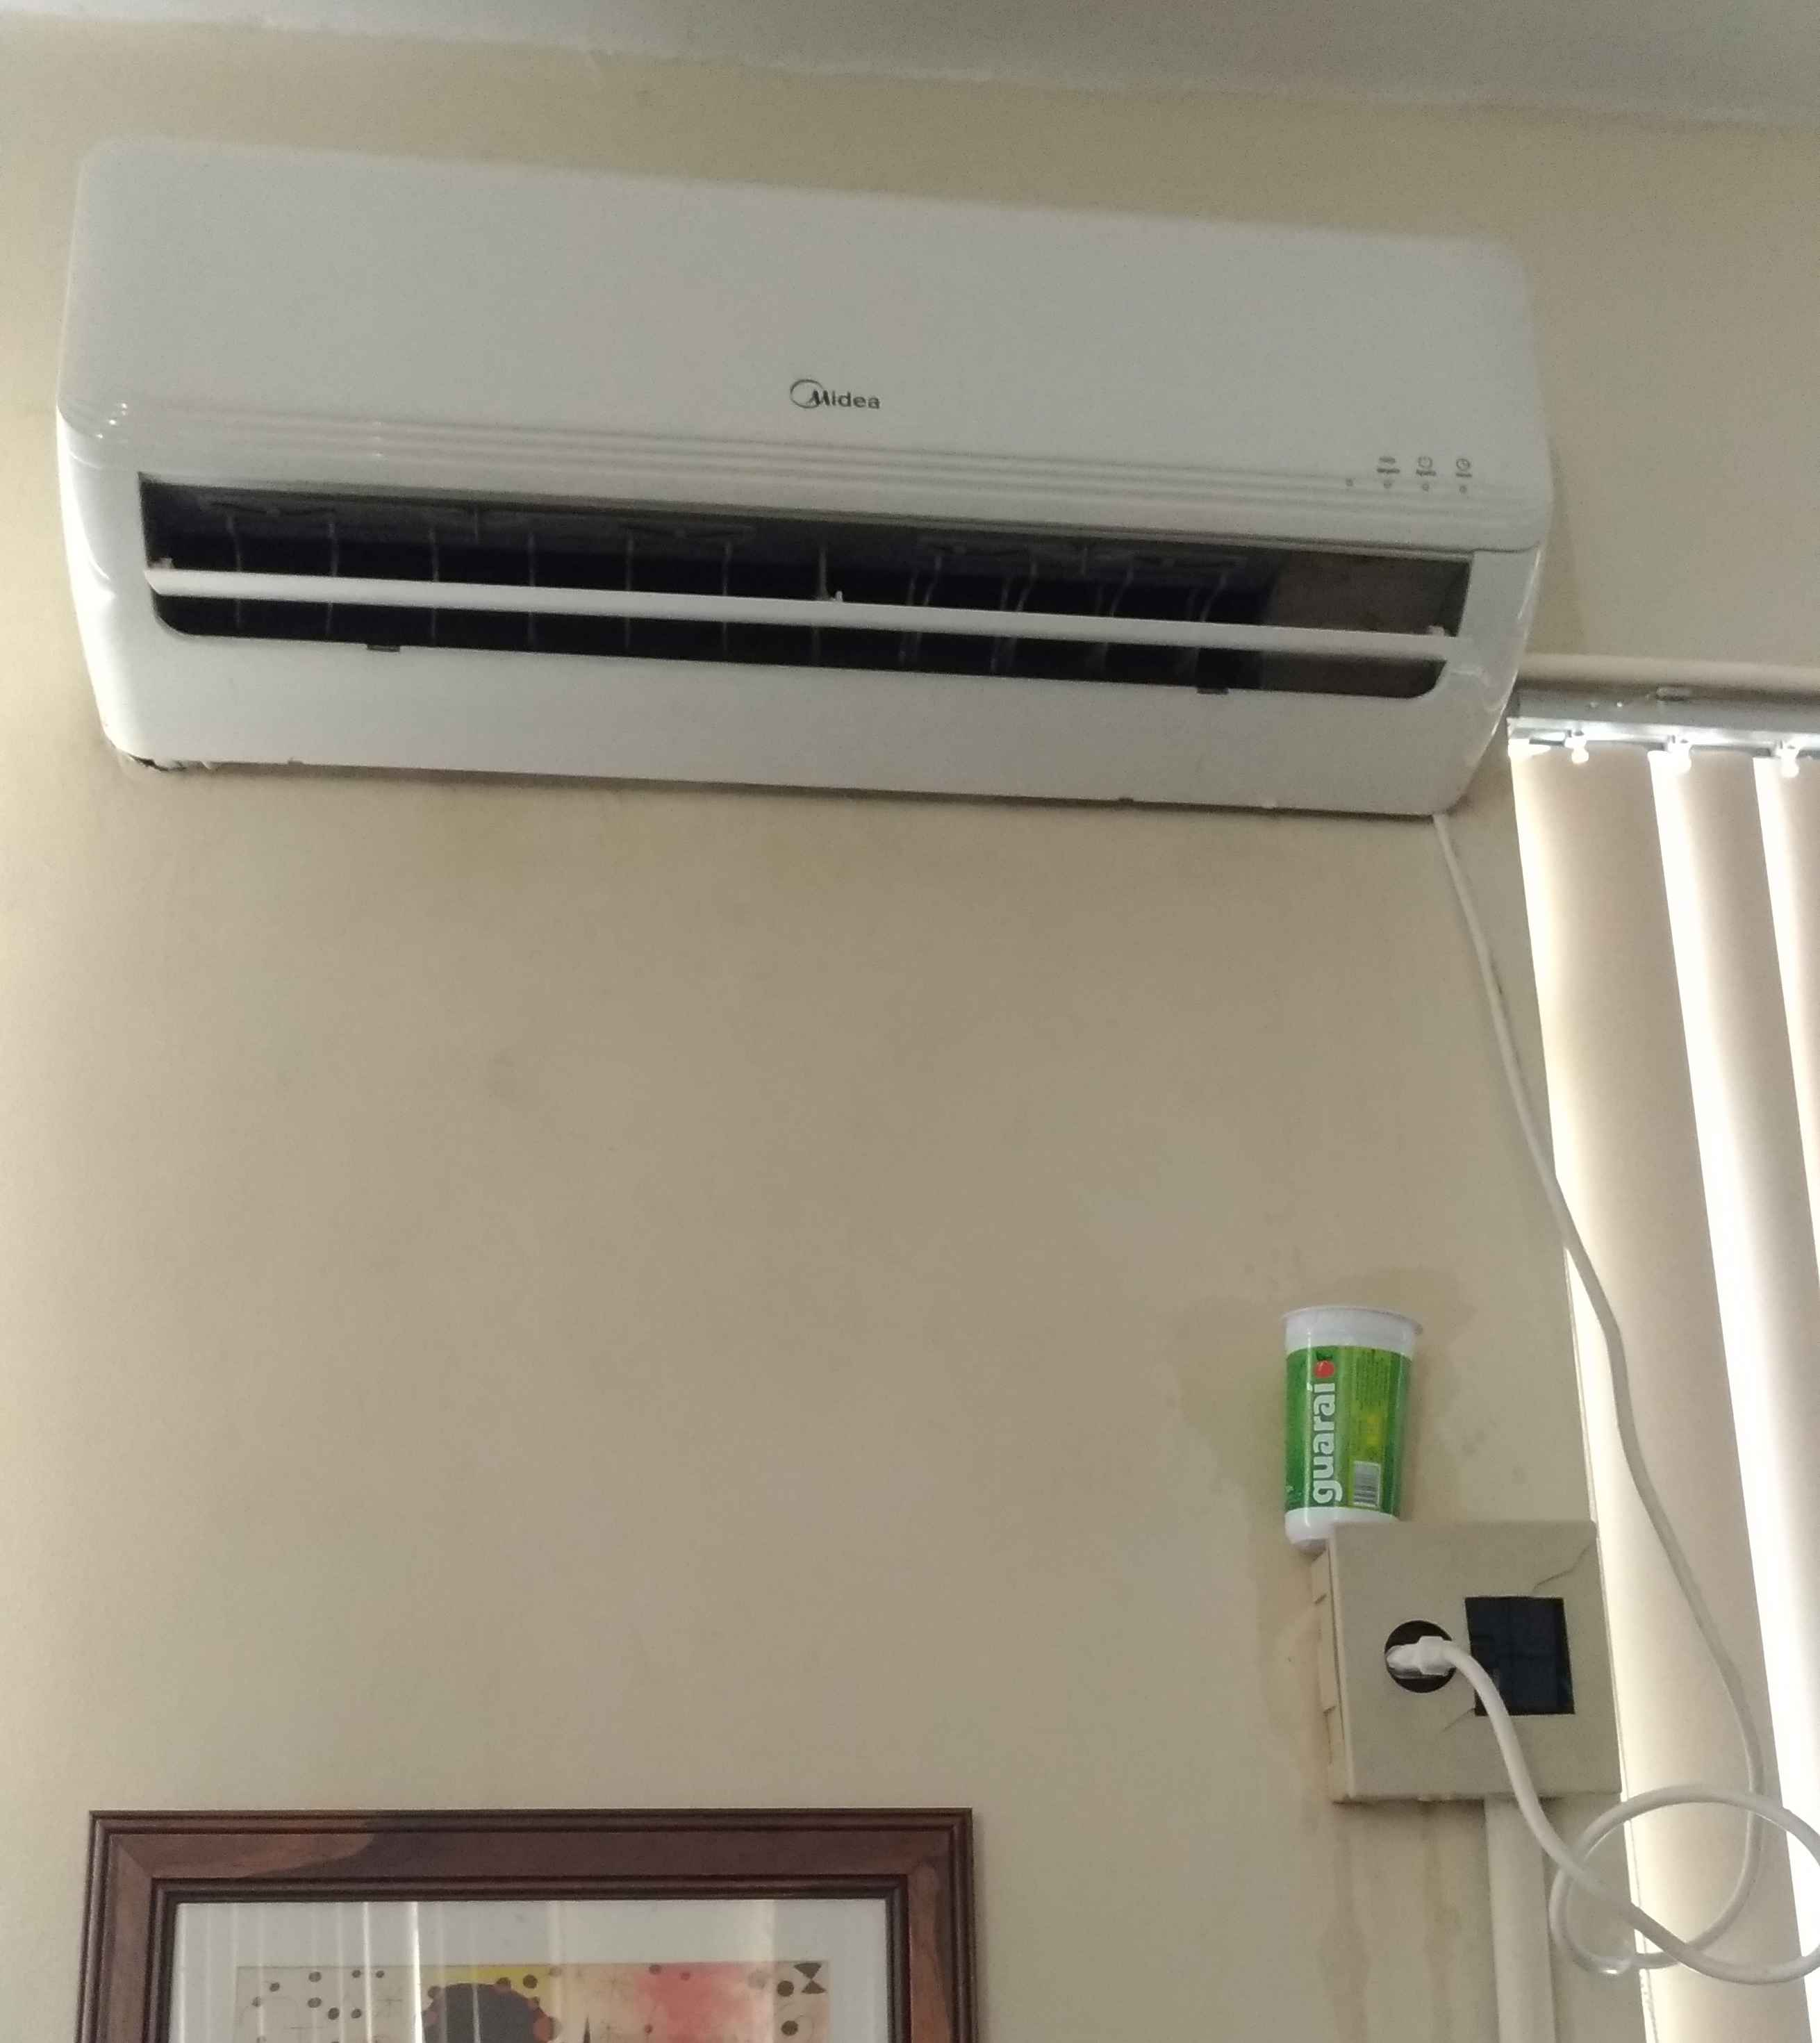
\includegraphics[width=0.7\textwidth]{imagens/copo.jpg}
  \caption{Ar condicionado pingando e copo sobre a tomada para coletar a água.}
  \label{fig:LABEL_FIG_COPO}
\end{figure}

A água que pingava e transbordava, então, havia molhado a caixa da tomada na qual o aparelho encontrava-se ligado naquele momento, bem como havia molhado o gabinete de um computador e uma das mesas dos computadores. Escorrendo pela parede para o chão, a água havia formado uma grande poça abaixo da mesa que fora molhada. A bolsista se mostrou chateada com a situação, reclamando, sozinha, quem alguém havia deixado o ar condicionado ligado ao sair do laboratório.

\begin{figure}[ht]
  \centering
  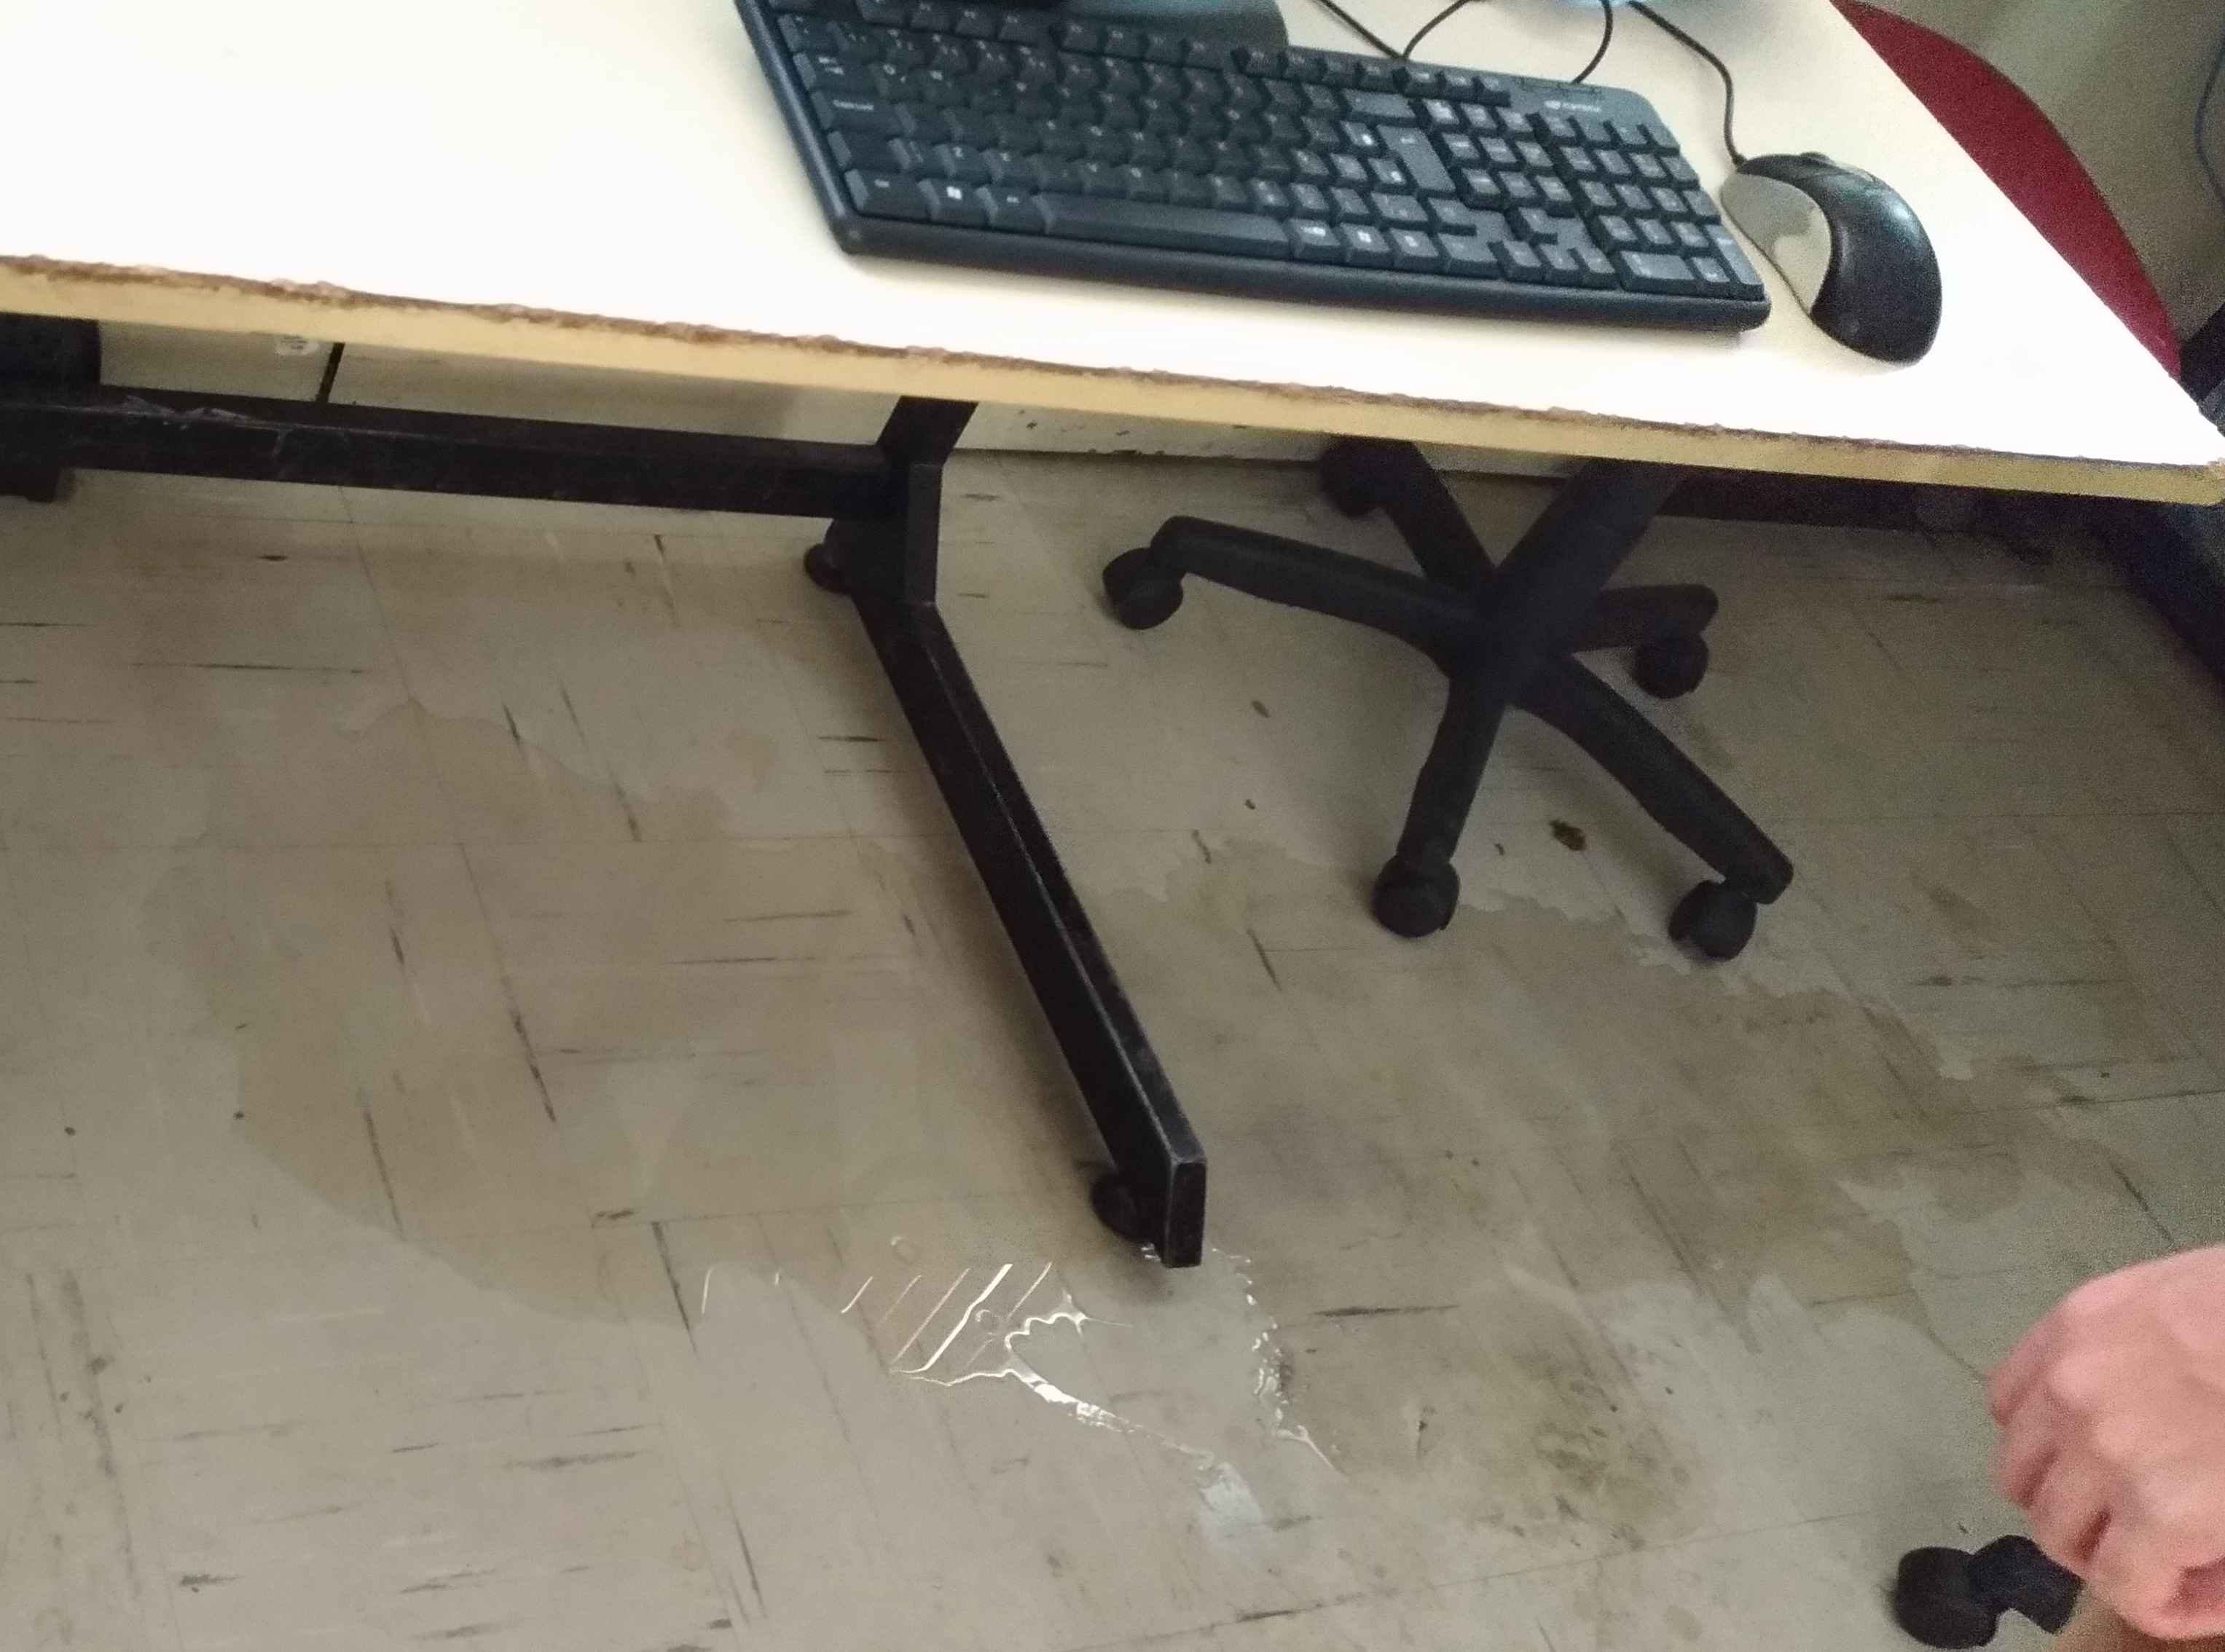
\includegraphics[width=0.9\textwidth]{imagens/poca.jpg}
  \caption{Poça formada no chão por conta do transbordamento do copo.}
  \label{fig:LABEL_FIG_POCA}
\end{figure}

Também foi observado que o laboratório possuía algumas cadeiras avariadas, com encosto e/ou assento rasgados, bem como uma cadeira cujo encosto havia sido removido, deixando os ferros que davam suporte ao encosto expostos, aumentando assim o risco de acidentes, principalmente com as crianças que frequentam o laboratório. 

Foi observado ainda que havia grande número de caixas de papelão, de conteúdo desconhecido, empilhadas atrás da porta do laboratório; e que a impressora do laboratório estava quebrada, com um papel anexado a ela, escrito “Em manutenção. Favor não ligar”.

Outra observação relevante é que o local onde o laboratório se encontra possui uma pilastra no meio da sala, o que dificulta o ministério de aulas. Além disso, foi possível observar colados nas paredes os avisos de relacionamento com o espaço que foram mencionados pela Profª. Isabel, da DALPE, na sua entrevista.

\begin{figure}[ht]
  \centering
  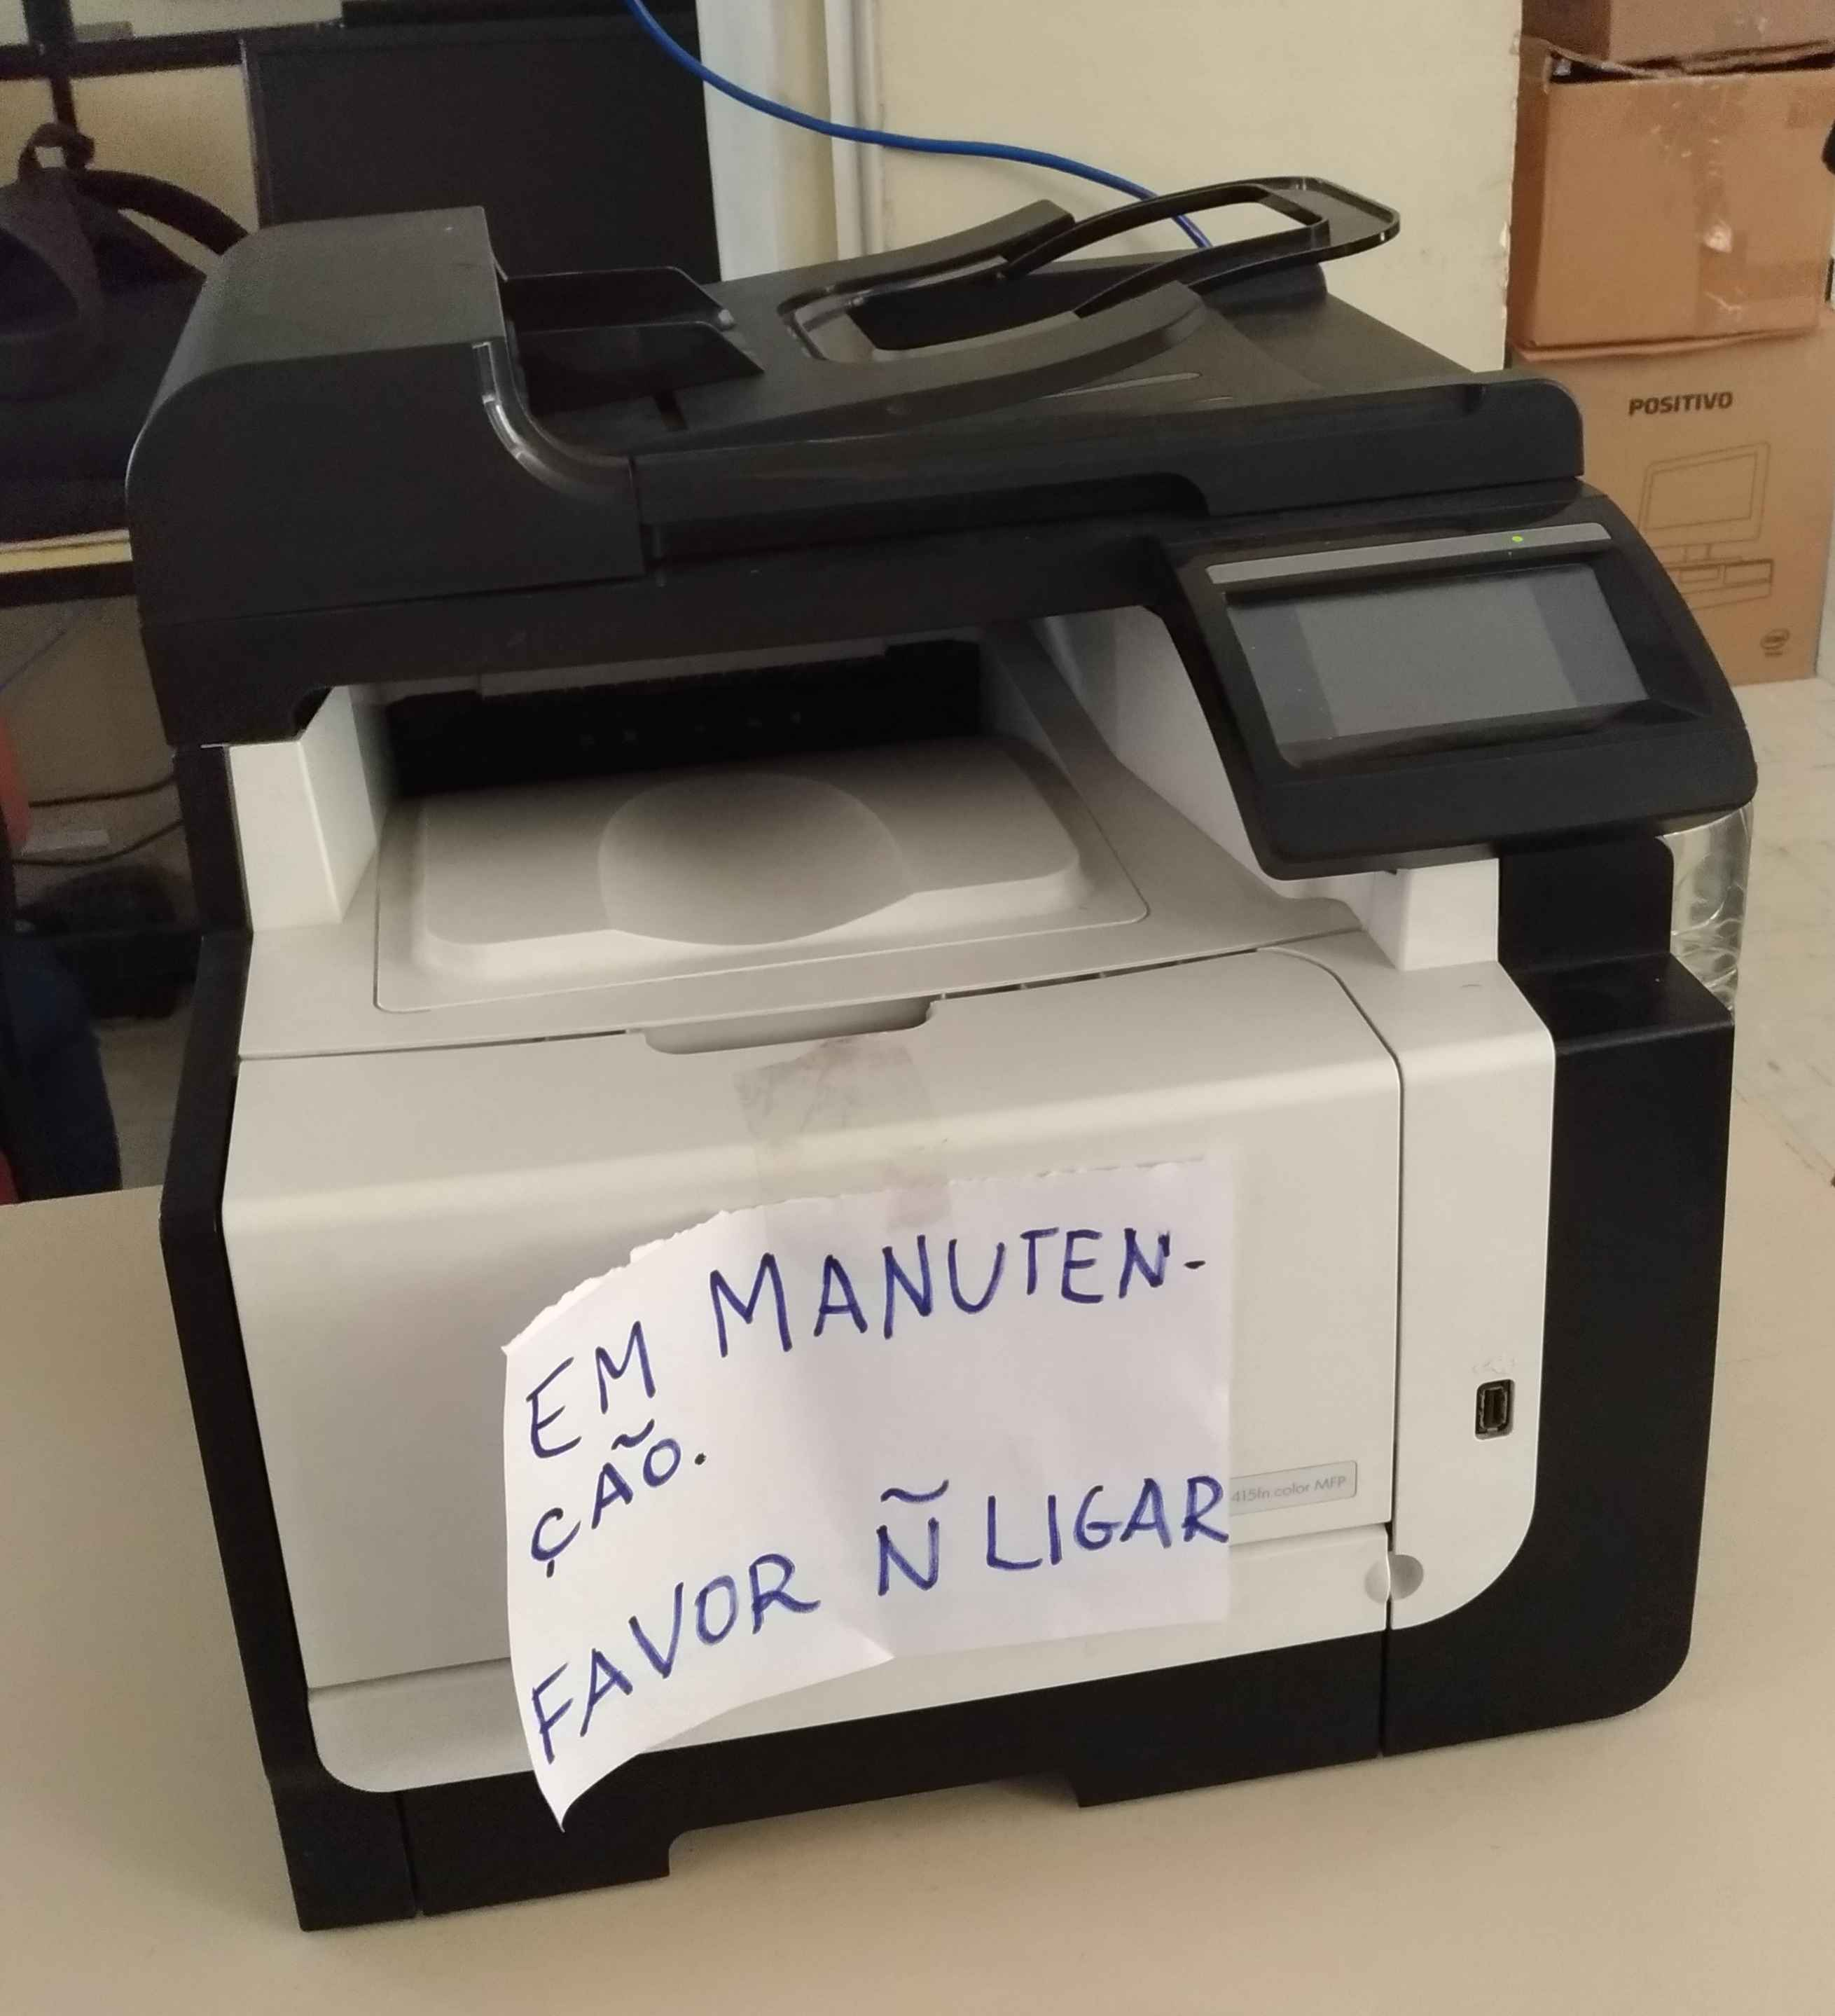
\includegraphics[width=0.8\textwidth]{imagens/impressora.jpg}
  \caption{Impressora com aviso de manutenção.}
  \label{fig:LABEL_FIG_IMP}
\end{figure}

\begin{figure}[ht]
  \centering
  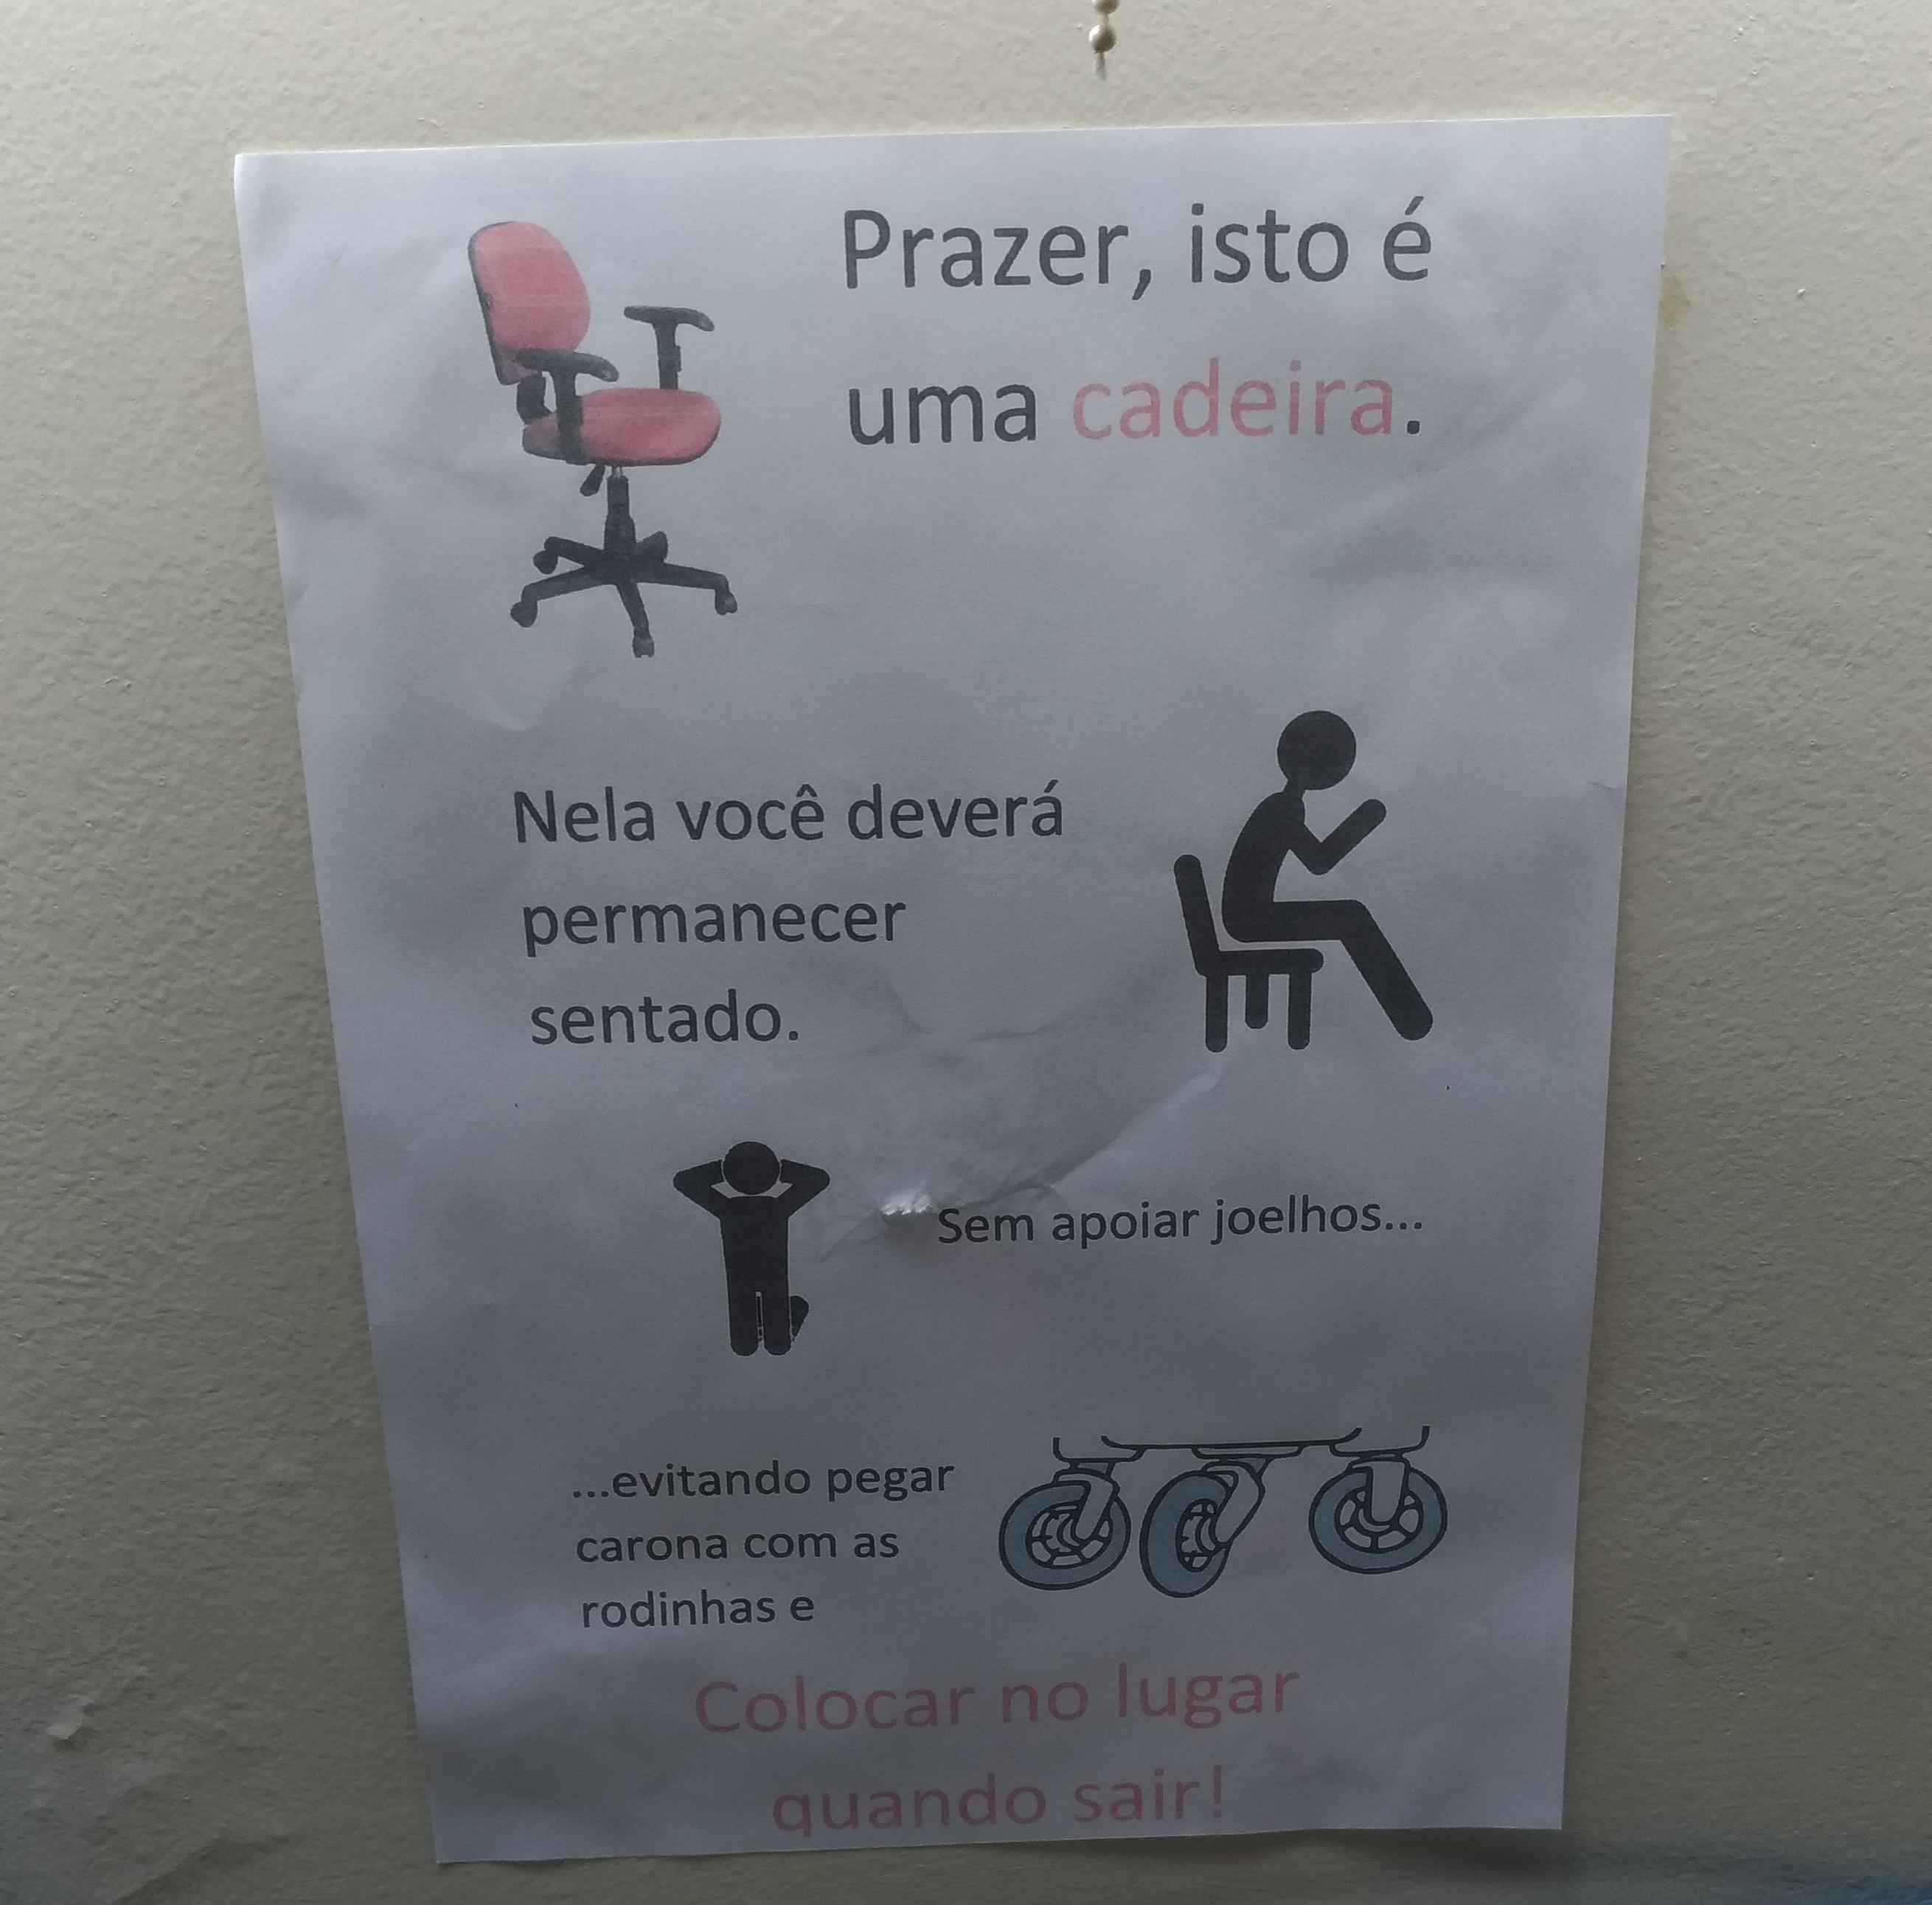
\includegraphics[width=0.8\textwidth]{imagens/aviso.jpg}
  \caption{Um dos avisos de relacionamento com o espaço.}
  \label{fig:LABEL_FIG_AVISO}
\end{figure}

% \subsection{A Chegada dos Alunos}\label{sec:LABEL_CHP_REL_SEC_REL_SUBSEC_CHEG_AL}

Neste momento, a professora Cassandra chegou com os alunos do 5º (quinto) ano para a aula. Ao acomodá-los no laboratório, foi necessário pedir para que as crianças tomassem cuidado com a área que estava molhada, e instruí-las no sentido de que não seria possível utilizar os computadores daquela área. Após acomodar todos os alunos no laboratório, ela pediu para que nós falássemos com eles. Bruno então informou-os de que não seria possível utilizar o laboratório naquele momento pois ainda estava faltando instalar o programa que seria utilizado por eles, o que gerou grande frustração nos alunos, que apresentavam visível empolgação com a perspectiva de assistir uma aula no laboratório.

Ao recolher os alunos para levá-los de volta à sala de aula, Cassandra informou que poderia voltar ao laboratório no 4º (quarto) tempo de aula, às 16h30min, caso o problema da instalação do software fosse solucionado em tempo hábil, ao que nos comprometemos em envidar esforços neste sentido.

% \subsection{A Chegada da Manutenção}\label{sec:LABEL_CHP_REL_SEC_REL_SUBSEC_CHEG_MAN}

Enquanto os alunos estavam no laboratório, o funcionário da manutenção que fora convocado para sanar o problema da porta interna trancada chegou, munido de uma escada de madeira e um cabo de vassoura. Devido à presença das crianças no laboratório, ele aguardou até que pudesse realizar seu trabalho. Após a retirada delas, posicionou a escada contra a porta e, subindo nela, comentou com a bolsista: “de novo essa porta, é?”.

Interpelada, a bolsista informou que não era a primeira vez que este problema acontecia; ao contrário, era um problema recorrente, e questionada acerca do porquê da DALPE não possuir uma cópia da chave, ela não soube explicar; questionado, o funcionário informou que o setor de manutenção não possui cópia daquela chave, mas também não deu explicações do porquê. A bolsista ainda informou que os seguranças do CAp, que guardam a chave do laboratório quando este não está em uso, também não possuem cópia da chave da porta interna.

Uma vez no topo da escada, o funcionário pegou o cabo de vassoura e passou-o por uma abertura acima da porta, de modo que este alcançasse a maçaneta pelo lado de dentro. Após alguns minutos de esforço, o funcionário conseguiu abrir a porta por dentro e deixou o recinto levando a escada e o cabo de vassoura, retornando logo em seguida com um pano de chão e um balde, para secar a poça d’água formada pelo ar condicionado que estava pingando.

Questionado se o problema era recorrente, ele disse que era bastante frequente que os bolsistas esquecessem de esvaziar o copo que coletava as gotas que pingavam e este transbordasse, formando assim a poça no chão e molhando os objetos ao redor do aparelho. A bolsista presente aproveitou a ocasião para esvaziar o copo. 

% \subsection{A Tentativa de Instalação do Software}\label{sec:LABEL_CHP_REL_SEC_REL_SUBSEC_INST}

Logo em seguida, questionamos a bolsista acerca da instalação do \textit{JFractionLab}, ao que fomos informados de que não seria possível realizá-la pois ela não possuía a senha de administrador das máquinas. A bolsista orientou-nos no sentido de que a instalação de novos programas deveria ser realizada por meio de solicitação à DALPE, e que, caso a solicitação fosse aprovada, os bolsistas se encarregariam de realizar a instalação dos programas solicitados e de informar quando o laboratório estaria disponível para utilização com estes programas.

Interpelada a respeito de quem seria responsável por realizar a avaliação técnica da solicitação de instalação de software, uma vez que a DALPE não possui funcionário com tal competência, a bolsista informou que um outro bolsista, o que possui a senha de administrador, faria a avaliação e aprovação ou não da solicitação, bem como o procedimento de instalação no caso de aprovação.

Uma vez que ficou claro que a decisão estava na mão de um bolsista, Filipe, que possuía o telefone deste bolsista, perguntou se seria possível realizar a instalação do programa obtendo uma autorização por telefone, ao que a bolsista que estava no laboratório aquiesceu, com a restrição de que a instalação fosse realizada por nós, alunos de computação, pois ela era aluna de um curso não relacionado à informática e não julgava possuir as competências técnicas necessárias para o procedimento de instalação.

Efetuada a ligação para o bolsista responsável pelas instalações de software e explicada a situação, a autorização foi concedida e a senha de administrador foi passada para a bolsista do horário, que a colocou em uma das máquinas para que a instalação fosse realizada. Realizamos, então, este procedimento, entretanto, a instalação não foi concluída com êxito, pois o \textit{JFractionLab} precisa de um software adicional para funcionar: o \textit{Java}.

Ao ser informada da situação, a bolsista disse que o \textit{Java} poderia ser instalado somente mediante autorização do outro bolsista. Em nova ligação telefônica, explicada a situação, o bolsista recusou o pedido de instalação, alegando que as máquinas não possuíam capacidade de hardware suficiente para rodar o \textit{Java}. Filipe questionou tal decisão, uma vez que Bruno já havia obtido um relatório do hardware da máquina à qual tinham acesso de administrador, e este relatório demonstrava a plena capacidade de hardware daquela máquina para atender os requisitos necessários à instalação do \textit{Java}; entretanto, o bolsista foi irredutível, solicitou que o telefone fosse passado para a bolsista do horário e a orientou no sentido de não permitir a instalação do \textit{Java}. Questionado acerca da presença, na máquina, de outros softwares instalados que possuíam requisitos técnicos superiores ao \textit{Java}, o bolsista não deu quaisquer explicações e se manteve irredutível.

% \subsection{A Procura por Alternativas}\label{sec:LABEL_CHP_REL_SEC_REL_SUBSEC_PROC_ALT}

Começamos então a avaliar alternativas que pudessem executar o \textit{JFractionLab} sem a presença do \textit{Java}. Inicialmente, pensamos em procurar o software em algum site de jogos, de modo que ele rodasse em um navegador, e, se não encontrássemos, tentar hospedá-lo em algum servidor que possuísse o \textit{Java}; entretanto, esta alternativa rapidamente se revelou inviável, pois os softwares em \textit{Java} que rodam em navegadores dependem de um \textit{plug-in}, que por sua vez depende da instalação do \textit{Java}.

Foi avaliada então a alternativa de realizar uma portabilidade automática de código fonte para uma outra linguagem, uma vez que o \textit{JFractionLab} é software livre e possui código aberto. Uma vez que o software estivesse em outra linguagem, seria possível executá-lo sem a presença do \textit{Java}.

Entretanto, os serviços de portabilidade automática encontrados se limitavam a programas pequenos, a menos que fosse realizada a compra de pacotes \textit{premium}, e o \textit{JFractionLab} possui código fonte muito extenso, inviável de ser portado utilizando os planos gratuitos oferecidos por esses serviços.

Além disso, uma pesquisa revelou que os programas portados utilizando esses serviços em geral resultavam em programas com muitos erros, que precisavam ser consertados manualmente, o que levaria muito tempo e não daria qualquer garantia de que o software portado funcionaria da mesma forma que o original, tornando, então, esta alternativa inviável.

Diante da falta de alternativas, informamos à professora Cassandra que não seria possível utilizar o laboratório naquele dia. Realizamos, então, a entrevista com a bolsista presente no laboratório e retiramo-nos da escola mais ou menos às 17 horas.

\section{Dificuldades que Enfrentamos}\label{sec:LABEL_CHP_REL_SEC_PROBS}

\subsection{O Atraso da bolsista}\label{sec:LABEL_CHP_REL_SEC_PROBS_SUBSEC_ATR}

A bolsista que deveria chegar às 13 horas chegou apenas às 13:45. Neste interstício, o laboratório permaneceu trancado, impossibilitando tanto a realização do trabalho a que nos propomos quanto o uso por parte dos alunos que procuraram o laboratório e o encontraram fechado.

% \subsubsection{Questionamentos levados ao CAp}
\begin{itemize}
    \item Questionamentos levados ao CAp
\end{itemize}

Vários bolsistas se atrasam, ou foi apenas esta bolsista? Esta bolsista se atrasa com frequência, ou foi um caso isolado? Os bolsistas atrasados sabem do impacto que podem causar ao laboratório ao se atrasarem?

% \subsubsection{Resposta do CAp}
\begin{itemize}
    \item Resposta do CAp
\end{itemize}

Os bolsistas eventualmente se atrasam por conta do deslocamento do Fundão (campus principal da UFRJ) para o colégio. Esse é o caso da Ingrid. Se tivesse sido realizado um contato anterior com ela, salientando a importância da pontualidade neste dia, a situação poderia ter sido contornada.

Cabe ressaltar que a posição do bolsista é de mero auxiliar das atividades do laboratório, e qualquer professor pode utilizá-lo sem a presença do bolsista, basta que solicite a chave. Dessa forma, o atraso de um bolsista não se configura, a princípio, como impeditivo para a realização de uma atividade no laboratório. Por conta disso, caso a presença dele seja imprescindível para a realização de uma atividade, isso deve ser avisado com antecedência. O simples fato de haver uma atividade marcada na planilha de aulas do laboratório não configura necessidade da presença do bolsista no laboratório.

\subsection{A Porta interna trancada}\label{sec:LABEL_CHP_REL_SEC_PROBS_SUBSEC_POR}

Na ocasião da chegada da bolsista foi constatado que a porta interna do laboratório, que dá acesso à área onde fica o computador utilizado pelos bolsistas e outros materiais relevantes, estava trancada, e o único bolsista que possuía a chave daquela porta já havia deixado o Colégio.

% \subsubsection{Questionamentos levados ao CAp}
\begin{itemize}
    \item Questionamentos levados ao CAp
\end{itemize}

Quem instalou a porta só forneceu uma cópia da chave? Por que essa cópia ficou com o bolsista, ou para quem foram dadas as outras? Quem é responsável por tirar cópias da chave? Por que essas cópias ainda não foram tiradas?

% \subsubsection{Resposta do CAp}
\begin{itemize}
    \item Resposta do CAp
\end{itemize}

A porta interna não possui fechadura, apenas maçaneta. Não sabemos o que ocorreu neste dia, mas pode ser que a porta estivesse apenas emperrada. A Ingrid é uma bolsista que está conosco há pouco tempo, talvez ela tenha se confundido e achado que a porta estava trancada.

\subsection{O Ar condicionado pingando}\label{sec:LABEL_CHP_REL_SEC_PROBS_SUBSEC_AC}

Um dos aparelhos de ar condicionado do laboratório está com um vazamento de água para a parte interna do laboratório. É um problema grave, pois está molhando tanto uma tomada, o que pode levar a um curto circuito e em último caso a um incêndio; quanto um computador, que é um equipamento caro.

% \subsubsection{Questionamentos levados ao CAp}
\begin{itemize}
    \item Questionamentos levados ao CAp
\end{itemize}

De quem é a responsabilidade de chamar a manutenção? Por que este responsável não chamou? Caso a manutenção já tenha sido chamada, por que ela não veio?

% \subsubsection{Resposta do CAp}
\begin{itemize}
    \item Resposta do CAp
\end{itemize}

A manutenção do ar condicionado do laboratório faz parte da manutenção de todos os aparelhos de ar condicionado da escola. No início de 2018 havia apenas um aparelho com defeito. Agora, quando voltamos às aulas em 2019, já temos sete aparelhos com defeito. Já foi realizado chamado de manutenção e esta será feita no sábado anterior ao carnaval, daqui a poucos dias.

\subsection{As Cadeiras avariadas}\label{sec:LABEL_CHP_REL_SEC_PROBS_SUBSEC_CAD}

Há diversas cadeiras avariadas dentro do laboratório, que podem causar acidentes e oferecem risco aos alunos que o utilizam.

% \subsubsection{Questionamentos levados ao CAp}
\begin{itemize}
    \item Questionamentos levados ao CAp
\end{itemize}

Por que cadeiras avariadas continuam dentro do laboratório? De quem é a responsabilidade de solicitar a troca das cadeiras? Este responsável solicitou a troca? Se sim, por que ela ainda não aconteceu?

% \subsubsection{Resposta do CAp}
\begin{itemize}
    \item Resposta do CAp
\end{itemize}

A substituição das cadeiras do laboratório será realizada quando houver cadeiras novas disponíveis. A compra de cadeiras novas já foi solicitada, e segue os mesmos trâmites das outras compras da UFRJ.

\subsection{As Caixas atrás da porta}\label{sec:LABEL_CHP_REL_SEC_PROBS_SUBSEC_CAIX}

Na ocasião da nossa visita, havia diversas caixas armazenadas atrás da porta do laboratório, prejudicando a circulação de pessoas, impedindo a abertura completa da porta e oferecendo risco em potencial às crianças.

% \subsubsection{Questionamentos levados ao CAp}
\begin{itemize}
    \item Questionamentos levados ao CAp
\end{itemize}

O conteúdo das caixas pertencia ao laboratório? Existe algum local no CAp destinado para armazenamento de caixas desse tipo?

% \subsubsection{Resposta do CAp}
\begin{itemize}
    \item Resposta do CAp
\end{itemize}

O conteúdo das caixas pertence ao laboratório, entretanto, nós temos muito pouco espaço no colégio como um todo, e não há outro local para armazenar as caixas.

\subsection{A Impressora quebrada}\label{sec:LABEL_CHP_REL_SEC_PROBS_SUBSEC_IMP}

Na ocasião da nossa visita, a impressora estava quebrada e sobre ela estava colada uma folha, na qual estava escrito: “Em manutenção. Favor não ligar”. Este problema impede o atendimento à forte demanda de impressões que chega ao laboratório, tanto da parte dos alunos, que precisam imprimir trabalhos; quanto da parte dos professores, que precisam imprimir provas.

% \subsubsection{Questionamentos levados ao CAp}
\begin{itemize}
    \item Questionamentos levados ao CAp
\end{itemize}

Quem é responsável por solicitar suporte e manutenção para a impressora? Quem realiza este suporte? A manutenção já foi solicitada? Se sim, por que a manutenção ainda não foi atendida pelo suporte?

% \subsubsection{Resposta do CAp}
\begin{itemize}
    \item Resposta do CAp
\end{itemize}

A manutenção da impressora já foi solicitada, entretanto a TIC/UFRJ (Superintendência de Tecnologia da Informação e Comunicação da Universidade Federal do Rio de Janeiro) possui poucos funcionários e muitos chamados, e até agora não conseguimos que o atendimento fosse realizado. Solicitamos também ao CFCH (Centro de Filosofia e Ciências Humanas), mas ele possui apenas um funcionário para manutenção na área de informática, e ele é responsável por todos os laboratórios e computadores administrativos do CFCH. Infelizmente a manutenção realmente demora a vir.

\subsection{A Pilastra no meio da sala}\label{sec:LABEL_CHP_REL_SEC_PROBS_SUBSEC_PIL}

Observamos nas entrevistas que os professores tem dificuldade de ministrar suas aulas no laboratório por conta da pilastra presente no meio da sala, que não permite que o professor tenha visão completa da turma enquanto ministra a aula. Foi levantada também a hipótese de que a pilastra na sala atua como fator desencorajador para que os professores utilizem o laboratório.

% \subsubsection{Questionamentos levados ao CAp}
\begin{itemize}
    \item Questionamentos levados ao CAp
\end{itemize}

Houve algum processo de decisão sobre o local do laboratório? Se sim, por que foi escolhida uma sala inadequada?

% \subsubsection{Resposta do CAp}
\begin{itemize}
    \item Resposta do CAp
\end{itemize}

A sala na qual o laboratório se encontra hoje é uma sala adaptada, e nós temos muito pouco espaço no colégio como um todo - há setores que não possuem sala para funcionar. Temos consciência de que a sala é inadequada para um laboratório, mas não há o que fazer. Não podemos construir mais salas pois o prédio onde funciona o colégio pertence à Prefeitura do Rio de Janeiro, e não à UFRJ.

\subsection{Somente um bolsista possui a senha de administrador}\label{sec:LABEL_CHP_REL_SEC_PROBS_SUBSEC_PSWD}

Na ocasião da nossa visita, foi-nos relatado pela bolsista do horário que a única pessoa que possui as senhas de administrador dos computadores é um bolsista. Além do risco de ter apenas uma pessoa de posse das senhas de administrador, o fato desta pessoa ser um bolsista deixa a administração técnica do laboratório a cargo de alguém que não possui vínculo com o colégio.

% \subsubsection{Questionamentos levados ao CAp}
\begin{itemize}
    \item Questionamentos levados ao CAp
\end{itemize}

Porquê apenas um bolsista possui a senha de administrador? A Direção Geral, DALPE ou outras coordenações sabem da senha de administrador? Existe alguma política para acesso a esta senha?

% \subsubsection{Resposta do CAp}
\begin{itemize}
    \item Resposta do CAp
\end{itemize}

Os bolsistas se organizam entre si com a senha de administrador, pois, por conta de não termos pessoal especializado para a manutenção do laboratório, esta acaba se tornando um encargo deles. Não exercemos maior controle sobre isso por falta de capacidade técnica.

\subsection{A Requisição de instalação de software é avaliada por um bolsista}\label{sec:LABEL_CHP_REL_SEC_PROBS_SUBSEC_REQ_INST}

Na ocasião da nossa visita, era necessário instalar um software nos computadores do laboratório, ao que nos foi informado que deveria ser realizada uma requisição de instalação de software, e que esta seria avaliada pelo bolsista que possui a senha de administrador. Por se tratar de uma decisão técnica relevante sobre o laboratório como um todo, esta deveria ser tomada por um profissional de formação comprovada, que possuísse vínculo com o CAp e fosse responsável pelo laboratório.

% \subsubsection{Questionamentos levados ao CAp}
\begin{itemize}
    \item Questionamentos levados ao CAp
\end{itemize}

Existe algum processo de avaliação formal de requisição de instalação de software, ou este fica apenas a cargo do bolsista?

% \subsubsection{Resposta do CAp}
\begin{itemize}
    \item Resposta do CAp
\end{itemize}

Não possuímos pessoal com a formação técnica necessária para avaliar as requisições de instalação de software, por isso elas ficam a cargo dos bolsistas. Não é o cenário ideal, mas foi dessa forma que conseguimos nos organizar.

\subsection{A Bolsista não possuía capacitação para instalar softwares nos computadores}\label{sec:LABEL_CHP_REL_SEC_PROBS_SUBSEC_INST_SOFT}

A bolsista que estava no laboratório quando estivemos nele nos relatou que não sabia instalar novos softwares nos computadores, o que é uma tarefa relativamente simples.

% \subsubsection{Questionamentos levados ao CAp}
\begin{itemize}
    \item Questionamentos levados ao CAp
\end{itemize}

Os bolsistas do laboratório necessitam de um conhecimento mínimo de informática para atuarem no CAp? Existe alguma capacitação básica dos bolsistas?

% \subsubsection{Resposta do CAp}
\begin{itemize}
    \item Resposta do CAp
\end{itemize}

A capacitação dos bolsistas é incentivada frequentemente, pois encaramos isso como uma maneira de complementar a formação deles, entretanto, nem todos os bolsistas tem conhecimentos técnicos, bem como nem todos os bolsistas tem conhecimentos pedagógicos. É por isso que, na seleção dos bolsistas, procuramos formar uma equipe multidisciplinar que atenda a todas as necessidades. A bolsista que esteve com vocês tem formação na área pedagógica, e não na técnica.

\section{O Que Aprendemos}\label{sec:LABEL_CHP_REL_SEC_CONC}

Quanto aos problemas mais estruturais, cuja solução não depende diretamente da atuação do CAp, como a manutenção do ar condicionado, onde a única saída é esperar que a manutenção venha, não vislumbramos solução mais imediata que esteja ao alcance de ser desenvolvida pelo CAp.

Entretanto, refletindo sobre os problemas expostos, chegamos à conclusão de que os que são de ordem técnica e pedagógica seriam sanados, ou pelo menos amenizados, com a presença do “docente do LIE”, um professor com formação tanto pedagógica quanto computacional, alocado para se responsabilizar pelo LIE e para transformar o laboratório em um verdadeiro recurso pedagógico no colégio.

Nesse contexto, o docente do LIE é responsável tanto pela manutenção do espaço e dos recursos tecnológicos quanto pela elaboração de projetos pedagógicos do laboratório, em consonância com o projeto pedagógico do colégio. O docente do LIE é responsável, ainda, por oferecer suporte tanto técnico quanto pedagógico aos professores que utilizarem o laboratório. Atualmente, no CAp, esse suporte, quando existe, é ineficaz; e o projeto pedagógico do laboratório é inexistente. Em poucas palavras, o docente do LIE é responsável por fazer a conexão entre as disciplinas do currículo regular e os recursos tecnológicos presentes no colégio.

\chapter{Plano de Ação}\label{chp:LABEL_CHP_CONC}

% \section{Introdução}\label{chp:LABEL_CHP_CONC_SEC_INTRO}

A partir das dificuldades encontradas, que foram relatadas no capítulo anterior, pudemos perceber que o uso do LIE é uma tarefa relativamente complicada e difícil mesmo para os docentes da própria instituição, que, além de não encontrarem suporte extensivo do ponto de vista técnico e pedagógico, ainda precisam lidar com dificuldades que acabam se tornando barreiras à utilização do laboratório, e que atuam, naturalmente, como fator desmotivador a esta utilização.

Percebemos, assim, que fomentar o uso do laboratório por parte dos docentes é um objetivo mais importante do que pensáramos a princípio, e que esse fomento deve começar com a tentativa de amenizar as dificuldades que o laboratório enfrenta e, assim, suavizar as barreiras nas quais estas se constituem.

Refletindo sobre o que aprendemos no referencial teórico e sobre as dificuldades encontradas, chegamos à conclusão de que a maioria delas seria sanada, ou pelo menos amenizada, com a presença do "docente do LIE" no laboratório do CAp.

Neste sentido, optamos por elaborar uma conclusão diferente da que imaginamos anteriormente para este trabalho, atendendo melhor ao objetivo de fomentar o uso do LIE entre os docentes do CAp-UFRJ.

\section{Avaliação das Possibilidades}\label{chp:LABEL_CHP_CONC_SEC_POSS}

Para que alguém assuma a posição de docente do LIE no CAp-UFRJ, vislumbramos duas possibilidades: a de deslocar um funcionário da escola, preferencialmente um professor, para esta função, que seria a opção preferencial, por ser menos burocrática e ter trâmite mais célere; ou a de contratar um professor especialmente para este cargo.

Apresentamos as opções à DALPE em uma reunião para colher \textit{feedback} a respeito das possibilidades de implementação das soluções por parte do CAp. Foi-nos dito que não há possibilidade de deslocar algum funcionário para esta função pois, por força contratual, a carreira dos professores já possui divisões de carga horária, que seriam violadas caso houvesse tal deslocamento.

Entretanto, a DALPE mostrou-se favorável à possibilidade de contratar um novo funcionário para assumir a posição de docente do LIE. Neste contexto, para dar suporte a esta contratação, decidimos por delinear os encargos, a formação necessária e a carga horária relacionados à função de docente do LIE, bem como tecer considerações a respeito de como deve se dar a sinergia entre este e os demais atores.

\section{O Cargo de Docente do LIE}\label{chp:LABEL_CHP_CONC_SEC_DOC}

\subsection{Encargos}\label{chp:LABEL_CHP_CONC_SEC_DOC_SUBSEC_ENC}

A seguir, enumeramos de maneira mais detalhada os encargos do docente do LIE:

\begin{itemize}
\item Zelar pelas condições de uso do laboratório, tanto realizando manutenção preventiva e corretiva de hardware e de software nos computadores, quanto monitorando o uso por parte dos alunos (ex.: estar atento a comportamentos agressivos ou que possam comprometer a infra-estrutura do laboratório). Estima-se que, por semana, o docente deva dedicar em torno de 3 (três) horas para esta atividade.

\item Zelar pelas condições do espaço do laboratório (ar condicionado, iluminação, televisão, infra-estrutura). Gerar relatórios para a DALPE solicitando o que for necessário (ex.: manutenção do ar condicionado). Estima-se que, por semana, o docente deva dedicar em torno de 1 (uma) hora para esta atividade.

\item Oferecer aos professores o suporte técnico necessário em relação à instalação e ao uso dos softwares desejados pelos mesmos. Estima-se que, por semana, o docente deva dedicar em torno de 4 (quatro) horas para esta atividade.

\item Oferecer aos professores o suporte pedagógico necessário para otimizar o uso do laboratório nas suas aulas, desde a etapa do planejamento até a execução (ex.: auxiliar no planejamento das aulas considerando as limitações do laboratório e os objetivos pedagógicos pensados pelo professor, auxiliar o professor na execução das aulas lidando diretamente com os alunos, etc). Estima-se que, por semana, o docente deva dedicar em torno de 4 (quatro) horas para esta atividade.

\item Elaborar propostas pedagógicas de uso do laboratório em projetos multidisciplinares, de modo a envolver a escola como um todo neste uso (ex.: feira de ciências). Estima-se que, por semana, o docente deva dedicar em torno de 4 (quatro) horas para esta atividade.

\item Gerenciar os bolsistas do laboratório. Esta atribuição envolve definir o perfil desejado para o bolsista, realizar o processo seletivo, distribuir tarefas, gerenciar escala de horários, gerenciar frequência de trabalho, avaliar a execução das tarefas, realizar reuniões de acompanhamento, entre outras atividades inerentes à gerência de bolsistas. Estima-se que, por semana, o docente deva dedicar em torno de 4 (quatro) horas para esta atividade.
\end{itemize}

\subsection{Formação Acadêmica}\label{chp:LABEL_CHP_CONC_SEC_DOC_SUBSEC_FORM_ACAD}

Para estar de acordo com o perfil desejado e ser capaz de cumprir com os encargos supracitados, é necessário que o funcionário que irá assumir a função de docente do LIE possua formação acadêmica adequada. Consideramos que o funcionário a ser selecionado atingirá o perfil desejado se possuir, no mínimo, uma das seguintes formações:

\begin{itemize}
\item Curso de graduação em Licenciatura em Informática;

\item Curso de graduação em qualquer Licenciatura ou curso de graduação em Pedagogia ou curso de graduação na área de Computação, acrescido de curso de pós-graduação na área de Informática Educativa.
\end{itemize}

Caso o funcionário, após assumir a função de docente do LIE, observar dificuldades na realização de alguma de suas atribuições, ele deve se sentir livre para realizar cursos de qualificação profissional ou de especialização, ato que deve ser incentivado e facilitado pelo CAp.

\subsection{Carga Horária}\label{chp:LABEL_CHP_CONC_SEC_DOC_SUBSEC_CAR_HOR}

Considerando as estimativas de horas que o docente deve dedicar a cada uma de suas atividades (vide enumeração detalhada dos encargos do docente, acima), recomenda-se que o docente do LIE tenha um regime de 20h semanais, e que alterne os horários nos quais estará presente, de modo que esteja no colégio em um dia na parte da manhã e no dia subsequente na parte da tarde. Os horários nos quais o docente não estiver no laboratório deverão ser preenchidos pelos bolsistas, de modo que estes possuam um horário em que estejam no laboratório sozinhos e um horário em que estejam no laboratório com a presença do docente, para que possa ser realizado o acompanhamento das atividades.

\subsection{Atribuições da DALPE e da DG}\label{chp:LABEL_CHP_CONC_SEC_DOC_SUBSEC_ATRIB}

É preciso ter em mente que, embora o docente do LIE seja soberano no uso do laboratório, ele está sujeito à administração escolar, que, na figura da DALPE e da DG, também possui atribuições, cujo cumprimento se faz necessário para o bom funcionamento do LIE.

Considerando que o Laboratório de Informática Educativa está subordinado à DALPE, o docente do LIE será lotado como funcionário deste setor, tendo como superior imediato o docente que estiver na chefia da DALPE, e tendo como setor superior a DG, conforme o organograma do CAp.

Neste contexto, é atribuição da DALPE observar o cumprimento das atribuições do docente do LIE e avaliá-las quanto ao alcance dos seus objetivos, bem como receber e analisar os relatórios provenientes do docente do LIE, e providenciar o atendimento às demandas identificadas pelo docente. Caso a demanda apresentada não esteja dentro da esfera de competências da DALPE, cumpre a esta atuar como interface entre o docente do LIE e a DG, encaminhando-a para ser solucionada.

Cabe à Direção Geral a solução de problemas estruturais e de outros problemas que venham a ser identificados pelo docente do LIE e encaminhados pela DALPE.

Conforme o exposto, fica evidente que a implementação da Informática Educativa no CAp é atribuição não apenas do docente do LIE, mas também da DALPE e da DG; e que a eficiência dessa implementação é intrinsecamente dependente da sinergia entre estes três atores.

\chapter{Conclusão}\label{chp:LABEL_CHP_CONC}

% \section{Introdução}\label{chp:LABEL_CHP_CONC_SEC_INTRO}

A partir das dificuldades encontradas, que foram relatadas no capítulo anterior, pudemos perceber que o uso do LIE é uma tarefa relativamente complicada e difícil mesmo para os docentes da própria instituição, que, além de não encontrarem suporte extensivo do ponto de vista técnico e pedagógico, ainda precisam lidar com dificuldades que acabam se tornando barreiras à utilização do laboratório, e que atuam, naturalmente, como fator desmotivador a esta utilização.

Percebemos, assim, que fomentar o uso do laboratório por parte dos docentes é um objetivo mais importante do que pensáramos a princípio, e que esse fomento deve começar com a tentativa de amenizar as dificuldades que o laboratório enfrenta e, assim, suavizar as barreiras nas quais estas se constituem.

Refletindo sobre o que aprendemos no referencial teórico e sobre as dificuldades encontradas, chegamos à conclusão de que a maioria delas seria sanada, ou pelo menos amenizada, com a presença do "docente do LIE" no laboratório do CAp.

Neste sentido, optamos por elaborar uma conclusão diferente da que imaginamos anteriormente para este trabalho, atendendo melhor ao objetivo de fomentar o uso do LIE entre os docentes do CAp-UFRJ.

\section{Avaliação das Possibilidades}\label{chp:LABEL_CHP_CONC_SEC_POSS}

Para que alguém assuma a posição de docente do LIE no CAp-UFRJ, vislumbramos duas possibilidades: a de deslocar um funcionário da escola, preferencialmente um professor, para esta função, que seria a opção preferencial, por ser menos burocrática e ter trâmite mais célere; ou a de contratar um professor especialmente para este cargo.

Apresentamos as opções à DALPE em uma reunião para colher \textit{feedback} a respeito das possibilidades de implementação das soluções por parte do CAp. Foi-nos dito que não há possibilidade de deslocar algum funcionário para esta função pois, por força contratual, a carreira dos professores já possui divisões de carga horária, que seriam violadas caso houvesse tal deslocamento.

Entretanto, a DALPE mostrou-se favorável à possibilidade de contratar um novo funcionário para assumir a posição de docente do LIE. Neste contexto, para dar suporte a esta contratação, decidimos por delinear os encargos, a formação necessária e a carga horária relacionados à função de docente do LIE, bem como tecer considerações a respeito de como deve se dar a sinergia entre este e os demais atores.

\section{O Cargo de Docente do LIE}\label{chp:LABEL_CHP_CONC_SEC_DOC}

\subsection{Encargos}\label{chp:LABEL_CHP_CONC_SEC_DOC_SUBSEC_ENC}

A seguir, enumeramos de maneira mais detalhada os encargos do docente do LIE:

\begin{itemize}
\item Zelar pelas condições de uso do laboratório, tanto realizando manutenção preventiva e corretiva de hardware e de software nos computadores, quanto monitorando o uso por parte dos alunos (ex.: estar atento a comportamentos agressivos ou que possam comprometer a infra-estrutura do laboratório). Estima-se que, por semana, o docente deva dedicar em torno de 3 (três) horas para esta atividade.

\item Zelar pelas condições do espaço do laboratório (ar condicionado, iluminação, televisão, infra-estrutura). Gerar relatórios para a DALPE solicitando o que for necessário (ex.: manutenção do ar condicionado). Estima-se que, por semana, o docente deva dedicar em torno de 1 (uma) hora para esta atividade.

\item Oferecer aos professores o suporte técnico necessário em relação à instalação e ao uso dos softwares desejados pelos mesmos. Estima-se que, por semana, o docente deva dedicar em torno de 4 (quatro) horas para esta atividade.

\item Oferecer aos professores o suporte pedagógico necessário para otimizar o uso do laboratório nas suas aulas, desde a etapa do planejamento até a execução (ex.: auxiliar no planejamento das aulas considerando as limitações do laboratório e os objetivos pedagógicos pensados pelo professor, auxiliar o professor na execução das aulas lidando diretamente com os alunos, etc). Estima-se que, por semana, o docente deva dedicar em torno de 4 (quatro) horas para esta atividade.

\item Elaborar propostas pedagógicas de uso do laboratório em projetos multidisciplinares, de modo a envolver a escola como um todo neste uso (ex.: feira de ciências). Estima-se que, por semana, o docente deva dedicar em torno de 4 (quatro) horas para esta atividade.

\item Gerenciar os bolsistas do laboratório. Esta atribuição envolve definir o perfil desejado para o bolsista, realizar o processo seletivo, distribuir tarefas, gerenciar escala de horários, gerenciar frequência de trabalho, avaliar a execução das tarefas, realizar reuniões de acompanhamento, entre outras atividades inerentes à gerência de bolsistas. Estima-se que, por semana, o docente deva dedicar em torno de 4 (quatro) horas para esta atividade.
\end{itemize}

\subsection{Formação Acadêmica}\label{chp:LABEL_CHP_CONC_SEC_DOC_SUBSEC_FORM_ACAD}

Para estar de acordo com o perfil desejado e ser capaz de cumprir com os encargos supracitados, é necessário que o funcionário que irá assumir a função de docente do LIE possua formação acadêmica adequada. Consideramos que o funcionário a ser selecionado atingirá o perfil desejado se possuir, no mínimo, uma das seguintes formações:

\begin{itemize}
\item Curso de graduação em Licenciatura em Informática;

\item Curso de graduação em qualquer Licenciatura ou curso de graduação em Pedagogia ou curso de graduação na área de Computação, acrescido de curso de pós-graduação na área de Informática Educativa.
\end{itemize}

Caso o funcionário, após assumir a função de docente do LIE, observar dificuldades na realização de alguma de suas atribuições, ele deve se sentir livre para realizar cursos de qualificação profissional ou de especialização, ato que deve ser incentivado e facilitado pelo CAp.

\subsection{Carga Horária}\label{chp:LABEL_CHP_CONC_SEC_DOC_SUBSEC_CAR_HOR}

Considerando as estimativas de horas que o docente deve dedicar a cada uma de suas atividades (vide enumeração detalhada dos encargos do docente, acima), recomenda-se que o docente do LIE tenha um regime de 20h semanais, e que alterne os horários nos quais estará presente, de modo que esteja no colégio em um dia na parte da manhã e no dia subsequente na parte da tarde. Os horários nos quais o docente não estiver no laboratório deverão ser preenchidos pelos bolsistas, de modo que estes possuam um horário em que estejam no laboratório sozinhos e um horário em que estejam no laboratório com a presença do docente, para que possa ser realizado o acompanhamento das atividades.

\subsection{Atribuições da DALPE e da DG}\label{chp:LABEL_CHP_CONC_SEC_DOC_SUBSEC_ATRIB}

É preciso ter em mente que, embora o docente do LIE seja soberano no uso do laboratório, ele está sujeito à administração escolar, que, na figura da DALPE e da DG, também possui atribuições, cujo cumprimento se faz necessário para o bom funcionamento do LIE.

Considerando que o Laboratório de Informática Educativa está subordinado à DALPE, o docente do LIE será lotado como funcionário deste setor, tendo como superior imediato o docente que estiver na chefia da DALPE, e tendo como setor superior a DG, conforme o organograma do CAp.

Neste contexto, é atribuição da DALPE observar o cumprimento das atribuições do docente do LIE e avaliá-las quanto ao alcance dos seus objetivos, bem como receber e analisar os relatórios provenientes do docente do LIE, e providenciar o atendimento às demandas identificadas pelo docente. Caso a demanda apresentada não esteja dentro da esfera de competências da DALPE, cumpre a esta atuar como interface entre o docente do LIE e a DG, encaminhando-a para ser solucionada.

Cabe à Direção Geral a solução de problemas estruturais e de outros problemas que venham a ser identificados pelo docente do LIE e encaminhados pela DALPE.

Conforme o exposto, fica evidente que a implementação da Informática Educativa no CAp é atribuição não apenas do docente do LIE, mas também da DALPE e da DG; e que a eficiência dessa implementação é intrinsecamente dependente da sinergia entre estes três atores.

\section{Considerações Finais}\label{chp:LABEL_CHP_CONC_SEC_CONS_FIN}

Embora nosso trabalho não tenha prosseguido da maneira planejada e não tenha chegado às conclusões que imagináramos em princípio, acreditamos que pudemos dar boas contribuições para o CAp-UFRJ.

Foi-nos relatado pela DALPE que já está em estudo a possibilidade de realização de \textit{workshops} para os professores a respeito do uso do laboratório na educação, com propostas pedagógicas que utilizem a informática, e que essa proposta surgiu em reuniões e discussões que foram desdobramentos das nossas visitas ao CAp e das entrevistas que realizamos com os atores envolvidos no laboratório.

Além disso, a demanda pelo docente do LIE nos foi apresentada nas entrevistas aos gestores, antes mesmo de concluirmos que este era o ator que faltava para um melhor funcionamento do laboratório. A conclusão deste trabalho, que apresenta o delineamento dos encargos do docente do LIE e a formação acadêmica necessária para exercer esta função, é uma contribuição importante pois fornece embasamento técnico a um eventual pedido de contratação de funcionário para ocupar esta função; bem como fornece embasamento bibliográfico consagrado, uma vez que a conclusão encontra sustento no referencial teórico apresentado.

\section{Trabalhos Futuros}\label{chp:LABEL_CHP_CONC_SEC_TRAB_FUT}

Se, por um lado, esperamos que a contratação do docente do LIE ocorra, por outro lado essa contratação não elimina a possibilidade de realização de mais trabalhos de naipe semelhante ao nosso no CAp. Existe a possibilidade de ser criado um projeto no qual alunos de computação possam prestar assistência técnica aos professores do CAp na elaboração de propostas pedagógicas que utilizem os recursos computacionais do laboratório.

Este projeto, além de ser uma boa contribuição para o CAp e para os seus professores, servirá ainda como complemento à formação acadêmica dos alunos dos cursos de computação, principalmente dos que se interessam pela área de Informática Educativa e que não encontram muitos ensejos de desenvolver suas aptidões pedagógicas.

A possibilidade de realização de um projeto nesta linha já está sendo analisada pelos professores do Departamento de Ciência da Computação da UFRJ, fruto do nosso contato com o CAp e da nossa parceria com os seus professores.

\pagebreak

%%%%%%%%%%%%%%%%%%%%%%%%%%%%%%%%%%%%%%%%%%%%%%%%%%%%%%%%%%%%
% B I B L I O G R A F I A
%%%%%%%%%%%%%%%%%%%%%%%%%%%%%%%%%%%%%%%%%%%%%%%%%%%%%%%%%%%%
% Retirar esta parte se o trabalho não tiver bibliografia
\makebibspage{abnt}{elementos-postextuais/referencias} % ESTA LINHA NÃO DEVE SER COMENTADA NA VERSÃO FINAL


%%%%%%%%%%%%%%%%%%%%%%%%%%%%%%%%%%%%%%%%%%%%%%%%%%%%%%%%%%%%
% G L O S S A R I O (opcional)
%%%%%%%%%%%%%%%%%%%%%%%%%%%%%%%%%%%%%%%%%%%%%%%%%%%%%%%%%%%%
% \makeglossarypage{\item [Palavra] Significado da palavra
}

%%%%%%%%%%%%%%%%%%%%%%%%%%%%%%%%%%%%%%%%%%%%%%%%%%%%%%%%%%%%
% A N E X O (opcional)
%%%%%%%%%%%%%%%%%%%%%%%%%%%%%%%%%%%%%%%%%%%%%%%%%%%%%%%%%%%%
\annex  % ESTA LINHA NÃO DEVE SER COMENTADA NA VERSÃO FINAL
\annexchapter{A - Entrevista com a Direção Geral}{}\label{anx:LABEL_ANX_A}

A presente entrevista foi realizada com a Professora Maria Cristina Miranda da Silva, Diretora Geral do CAp-UFRJ, no dia 18 de outubro de 2018. As perguntas realizadas estão grafadas em itálico.

\textit{Você acha importante, ou ao menos pertinente, o uso do laboratório?}

O uso do laboratório é importante no contexto escolar e pedagógico para que as disciplinas tenham apoio nos seus conteúdos. Cito meu próprio caso como exemplo, por ser professora de artes visuais: há várias questões em que pode se utilizar os computadores, usando softwares para pesquisas sobre arte ou para a própria “atividade fim”, a criação da arte visual.

O laboratório poderia ser um espaço em que o estudante ficasse no contraturno, para fazer trabalho ou realizar pesquisa, utilizando-o como apoio acadêmico. Entretanto, o laboratório não funciona como seria desejável. Dentre os diversos motivos, identifico dois centrais:

Não há funcionário específico para o laboratório. Trabalhamos com bolsistas, e esse trabalho é difícil, pois, por serem estudantes, os bolsistas não têm autoridade de funcionário para administrar esse laboratório.

Não existe uma cultura entre o corpo docente para utilizar o laboratório, pois o professor é co-responsável pela forma de trabalho. Ele não pode, por exemplo, ficar só com um aluno e deixar os outros sem supervisão. Uma cultura de regras e formas de utilização precisa ser pensada, e o projeto de vocês pode ajudar a construir essa cultura. Observamos problemas relacionados ao uso do laboratório, como alunos que escrevem que são fascistas no plano de fundo do computador, dentre outros. Temos 720 alunos no CAp, em média 30 por turma, não sei exatamente a capacidade do laboratório, mas ele não comporta todos os alunos de uma turma, e precisa ser trabalhado com frações dela; isso também é um problema na criação dessa cultura de utilização do laboratório.

\textit{O que compete ao gestor no uso do laboratório de informática?}

Compete ao gestor zelar pelo equipamento que está ali, pois ele é caro. Primeiro a compra, depois o zelo, e depois a manutenção. Compete ao gestor o acompanhamento do uso do equipamento, e também compete a ele solicitar os funcionários necessários. Considerando o “gestor” como “o grupo coletivo de trabalhadores com a responsabilidade da tarefa de gerir o laboratório”, também compete fazer a escolha dos programas que serão disponibilizados. No caso do CAp, compete à Direção Geral fazer a compra dos equipamentos e os pedidos de funcionários, bem como pedidos de infra-estrutura, como ar condicionado, mesas, etc. A DALPE é a que fica responsável pela “administração” do espaço. A mediação entre a administração e os professores e estudantes é feita pela DALPE e DAE. Não quer dizer que é assim sempre, em todos os lugares, nem que essa é a melhor forma de gestão, mas foi assim que o CAp se estruturou. 

\textit{Como você, como gestora do CAp, considerando as limitações às quais está sujeita, poderia promover o uso do laboratório?}

A questão de não haver um funcionário específico para o laboratório é fundamental, e compete à Direção Geral. O trabalho com os bolsistas é muito complicado, pois não há autoridade para o bolsista.

\textit{Autoridade para o bolsista em que sentido?}

Os bolsistas são jovens, estudantes, que não podem ser responsabilizados por coisas graves. O bolsista não é um funcionário, mas sim um estudante. Por exemplo, o CAp é um campo de estágio que recebe licenciandos, mas esses licenciandos não podem ficar sozinhos com os alunos. É necessário ter um funcionário da escola que se responsabilize por esse contato. O bolsista \textbf{auxilia} o processo, mas não pode ser responsável por ele. Isso é um problema na liberação do laboratório em tempo vago, por exemplo. No caso em que um professor precise faltar e não dê sua aula, as crianças não podem ir para o laboratório porque o bolsista não pode se responsabilizar pelo uso dele. É necessário ter um professor ou funcionário presente. Temos bolsistas cuidando do laboratório enquanto o funcionário cuida da turma, essa é a separação.

\textit{Como um gestor hipotético que disponha de todos os recursos que ele quiser poderia promover o uso do laboratório?}

Num cenário ideal a gente teria um laboratório maior, que comportasse a turma toda, com mais máquinas, uma por aluno, e com pelo menos dois funcionários, que pudessem atuar um na orientação do bolsista e outro na recepção do estudante, que fossem especialistas no assunto, formados em educação ou informática no ensino. Esses funcionários poderiam pensar o laboratório, fazer dele um projeto grande na escola, um projeto da escola como um todo, independente, montado pelos funcionários, com conhecimento pedagógico e de computação, com horário separado na grade. Alguém que use o laboratório não deve estar preocupado com computador que não liga, com puxar fio de tomada, essa pessoa precisa só utilizar o equipamento, sem se preocupar com a manutenção. Precisa ter um educador com essa perspectiva. O professor só vai no laboratório com os alunos para fazer uma pesquisa ou digitar algo. É preciso criar essa cultura de uso do laboratório, é preciso uma equipe que pense as finalidades, que divida a responsabilidade do laboratório nessa perspectiva técnica e didática.

\textit{Na sua graduação como professora, você teve contato com a informática? E com a informática voltada para a educação?}

Não tive disciplina de uso do computador na graduação porque fiz graduação há muito tempo, não existia computador pessoal naquela época (\textit{risos}); mas tive contato com o computador por fora. Fiz, inclusive, um curso no qual aprendi a programar em \textit{Basic}, mas cartão perfurado não era a minha praia. Gosto de artes visuais.
Hoje eu enxergo o computador como uma extensão do corpo, sabe? Eu fico pensando, se eu for presa, o que vou fazer na cadeia sem celular e computador? Se eu precisasse sobreviver, não me preocuparia com a comida, mas com a tecnologia (\textit{risos}).

\textit{E hoje, você sabe como é esse contato com a informática voltada para a educação nas graduações?}

Não sei, e fico curiosa para saber. Saber como a informática é tratada em cursos de pedagogia e licenciatura, se há disciplina de informática voltada para a educação, se há interesse em pensar nas mídias e no ensino. São duas coisas, uma é você aprender a utilizar a tecnologia como mediador, e outra é trabalhar a atividade fim, a educação. Para encerrar, deixo vocês com uma pergunta a ser pensada: atualmente as crianças “já nascem” sabendo usar a tecnologia. Hoje ainda cabe ensinar uma criança a mexer no computador?

\annexchapter{B - Entrevista com a Direção Adjunta de Licenciatura, Pesquisa e Extensão}{}\label{anx:LABEL_ANX_B}

A presente entrevista foi realizada com a Professora Isabel Van Der Ley Lima, Diretora Adjunta de Licenciatura, Pesquisa e Extensão do CAp-UFRJ, no dia 18 de outubro de 2018.

\textit{Quais são as propostas pedagógicas atuais para o uso do laboratório?}

Primeiro vou contar uma história: o Laboratório de Informática (LIG) fica ligado à DALPE, pelo regimento do CAp. Até o ano passado a Profª. Izabel estava aqui, e tinha conhecimentos tanto técnicos quanto pedagógicos. Eu e a Profª. Marilane (a outra diretora da DALPE) não temos essa familiaridade tão grande.

Hoje o uso do laboratório é basicamente para acolher as aulas. As propostas pedagógicas são desenvolvidas pelos professores dos setores, e às vezes elas não têm muito a ver com o uso da informática. Por exemplo, hoje um professor de línguas usou o laboratório para passar um filme, e não usou os computadores; então o uso é mais do espaço do que do laboratório, o que gera uma certa insatisfação da parte dos bolsistas.

A coordenação do LIG não tem proposta pedagógica específica, porém temos a proposta de que os bolsistas familiarizem os alunos no sentido de compreender o laboratório como espaço acadêmico público. É muito frequente que alunos, principalmente do Fundamental II, entrem no LIG e causem danos aos materiais, tanto físicos, como tirar teclas do teclado e brincar de ficar empurrando as cadeiras, quanto danos digitais, pois às vezes eles alteram a configuração do computador, e essa alteração impede o uso de outros colegas, aí os bolsistas precisam descobrir o que foi modificado para reverter; então tem sido trabalhado que os bolsistas conversem com os alunos no sentido de conscientizar sobre o uso do laboratório. Sugiro que vocês entrevistem o bolsista Marcos, o horário dele é segunda e quarta de manhã. Eu brinco dizendo que ele é o “coordenador dos bolsistas”, pois é o que tem mais acúmulo de experiências.

Quanto ao uso dos jogos, ele é livre, mas há um jogo específico que estava gerando muita discussão. Não sei qual jogo é, mas tem conteúdo violento, e os alunos ficavam muito exaltados. Isso interferia no uso físico do laboratório, então, depois de muita discussão, acabamos decidindo por bloquear esse jogo específico, mas o uso dos jogos em geral é livre. O que a gente tem trabalhado nesse sentido é colocar alguns avisos de relação com o laboratório como espaço acadêmico.

As propostas pedagógicas além disso ficam a cargo dos setores pedagógicos que utilizam o laboratório. Na minha opinião, a matemática é o setor que mais utiliza o laboratório com o intuito de pensar propostas pedagógicas para o ensino associadas à questão da informática. O professor Fernando Velar tem um projeto de pesquisa e extensão no laboratório com os alunos da educação básica, acho que o professor Cléber utilizou o laboratório para o mestrado também.

\textit{A matemática tem uma visão mais pedagógica, mas como as outras áreas utilizam o laboratório?}

Os bolsistas podem informar melhor quais áreas usam e com quais finalidades. Aqui na DALPE a gente não pede para o professor registrar o objetivo da proposta, pedimos apenas para ele marcar a aula, então quem percebe melhor essa questão são os bolsistas, que estão ali no dia a dia. Pelo que eles me dizem, a área que mais utiliza o laboratório com objetivo pedagógico ligado à tecnologia é a matemática. As outras áreas usam mais o espaço do laboratório do que o laboratório em si, como foi o caso do professor que usou o laboratório hoje para passar filme.

\textit{Você acha que uma proposta pedagógica unificada para todos, como sugestão, seria melhor do que propostas individuais?}

O LIG poderia propor usos pedagógicos mais gerais. Uma questão forte agora é a inclusão. Temos um aluno que é autista, e que faz muito uso do LIG com a professora que o acompanha, de educação especial. Seria legal pensar em como essa professora trabalha, para poder expandir esse trabalho. Estamos montando uma sala de recursos, que ficará ao lado do LIG, e estamos pensando na questão do uso da informática como recurso para inclusão.

Seria bom termos mais propostas pedagógicas, pois muitos professores não fazem uso do laboratório pois não relacionam o uso da tecnologia às aulas. Aqui no CAp os setores pedagógicos têm muita autonomia na construção dos seus trabalhos pedagógicos, embora exista o projeto da escola em si. A gente poderia propor uma proposta pedagógica maior, mais geral, embora isso não seja feito; mas mesmo com essa proposta depende de cada setor comprar ou não a ideia. As propostas precisam ser mais uma sugestão, e não algo que comprometesse o trabalho.

Gostaria de abordar também uma questão estrutural: o laboratório é pequeno e tem uma coluna no meio do caminho, o que dificulta para dar aula; então alguns professores optam por não ir pela dificuldade do espaço. O laboratório até comporta todos os alunos, mas turmas menores, ou frações de uma turma, costumam funcionar melhor. Os professores de línguas usam mais o laboratório porque suas turmas são menores.

\textit{Como é utilizado o laboratório?}

Todos os horários têm um bolsista, e o trabalho dele é supervisionar o uso do laboratório pelos alunos quando não está tendo aula, e oferecer suporte ao professor quando há aula. Na nossa percepção, os alunos do Fundamental II usam muito para jogar, e os do Ensino Médio usam mais para fazer trabalhos. Houve uma discussão sobre uso do laboratório pelo Fundamental I, para que eles o utilizassem apenas sob supervisão de professores (sem uso livre), mas o Fundamental II e o Ensino Médio têm acesso tanto livre quanto com professor. Os horários do recreio são os que têm maior procura.

\textit{Há quantos bolsistas?}

Atualmente temos 5 (cinco) bolsistas. Eles trabalham 8 (oito) horas, divididas em dois turnos. Podem ser duas manhãs, duas tardes, ou uma manhã e uma tarde.

\textit{Qual a viabilidade da realização de um projeto de extensão, por parte dos alunos da UFRJ, no laboratório?}

Seria ótimo um projeto de extensão. A prioridade do uso é das aulas, depois do uso livre, então, acontecendo um projeto, seria necessário reservar o uso do laboratório, para não haver conflito com as aulas, pois o professor do CAp é apegado às suas aulas e é difícil mudar planejamentos, então não pode haver conflitos, mas esse é o único requisito. A questão é marcar com antecedência para garantir o uso do laboratório.

Se vocês conversarem com os bolsistas, podem identificar o que é mais necessário, quais as maiores demandas, porque a minha percepção é indireta, através de reuniões eventuais entre a DALPE e os bolsistas, para avaliar determinadas situações.

\textit{Podemos participar dessa reunião?}

Ainda não temos dia e horário para a reunião, mas a próxima deve ser na semana que vem. Vocês podem deixar seus contatos que eu aviso.

\textit{Na sua graduação como professora, você teve contato com a informática? E com a informática voltada para a educação?}

Olha, meu primeiro computador foi um 486, vocês não devem nem saber o que é isso! (\textit{risos}). Eu fiz cursos de DOS e de Windows 3.1, mas fora da graduação. A UFRJ tinha muito pouco dinheiro no final da década de 90, quando eu fiz minha graduação, e a parte de informática era muito precária, então não houve contato com a informática, embora algumas matérias demandassem o uso do computador, como análise de dados, estatística, etc. Hoje eu acho que o LIG é mais funcional na Biologia da UFRJ. Agora, disciplina de informática voltada para a educação, nenhuma. Não houve diálogo entre informática e educação, mas hoje há disciplinas nessa linha no NUTES, lá no CCS, são optativas. Eles são legais, abertos ao diálogo, e fazem trabalhos com escolas.

Dentro da UFRJ, já como docente, eu tive contato com a informática na educação por causa do Prof. Fernando. Fomos ao NCE para verificar possibilidades de relacionar educação com tecnologia, mas institucionalmente nunca houve incentivo. Hoje a formação ainda tem pouco diálogo com isso, são mais iniciativas pontuais dos professores. Os currículos que eu tenho visto não oferecem esse diálogo.

Estou trabalhando no complexo de formação de professores da UFRJ, que propõe uma reestruturação dessa formação, e mesmo assim não vejo muitas discussões sobre tecnologia. Acho que temos tantos problemas que são tão mais básicos, como conciliar o horário do aluno, por exemplo; há cursos de licenciatura que não dialogam com o local onde ele faz estágio. Isso é uma coisa simples de ser feita e nós temos problemas, então a tecnologia acaba ficando um pouco de lado.

Há também uma questão estrutural da universidade. Por exemplo, não existe rede de informática aqui na DALPE, tudo foi feito na base do “puxadinho”. Recorri à TIC/UFRJ, e eles se mostraram abertos a fazer um projeto de rede, mas é necessário ter a planta baixa do local. Fui no setor responsável por isso, mas há dificuldade para obter essa planta pois o prédio não é da UFRJ, é cedido pela prefeitura.

O CAp não tem funcionário responsável pela parte de tecnologia, então outra coisa que eu verifiquei com a TIC/UFRJ foi a possibilidade de ter, mas não há disponibilidade, pois a própria TIC/UFRJ tem um número pequeno de funcionários para atender à Universidade como um todo, e não há como deslocar um funcionário para uma unidade. É difícil ter acesso a coisas em geral. Aqui no CAp só temos 3 (três) salas de aula com \textit{Datashow}, que é um recurso simples, só projeta uma imagem. Só há um funcionário relacionado à parte de áudio-visual.

Faltam profissionais que tenham formação não apenas na área de informática, mas na área de educação também. Essa é uma questão visível na seleção dos bolsistas: há bolsistas de Ciência da Computação que são ótimos técnicos, mas têm dificuldade no diálogo educacional; e há bolsistas com formação pedagógica que não sabem usar o computador. Por conta disso, tentamos estabelecer um diálogo entre eles para tentar complementar a formação de ambos. Temos uma bolsista que faz Licenciatura em Letras e tem conhecimentos de informática, mas por fazer disso uma fonte de renda e não por ter formação acadêmica para tal.

Eu vejo que há pouca interface de diálogo entre a tecnologia e a educação, tanto na UFRJ quanto em outros lugares, como a PUC-RJ, onde eu fiz doutorado, e é um trabalho muito necessário.

\textit{A PUC-RJ possui um Colégio de Aplicação também, não é?}

Sim, mas o colégio não é da PUC-RJ, é um convênio. Inclusive, eu tenho uma amiga que trabalha lá e tem uma disciplina que trabalha com tecnologias.

Eu fiz doutorado em educação na PUC-RJ. Quando eu estava saindo de lá, eles estavam contratando um professor para dialogar com a parte de educação e tecnologia, mas não sei se foi contratado mesmo, porque realmente falta gente que faça esse diálogo.

\annexchapter{C - Entrevista com a Profª. Cassandra}{}\label{anx:LABEL_ANX_C}

A presente entrevista foi realizada com a Professora Cassandra, que dá aulas de matemática para o Fundamental I, no dia 31 de outubro de 2018.

\textit{Você utiliza, ou já utilizou, o laboratório de informática do CAp?}

Não.

\textit{Por que você não utiliza o laboratório de informática? Gostaria de utilizá-lo? Quais motivações te levariam a sair da sala de aula e levar os alunos ao laboratório?}

Nunca utilizei o laboratório como professora, e nunca parei para pensar no porquê. Tenho o desejo de utilizar, mas nunca parei para planejar de fato uma aula lá. Tenho esse desejo porque sei dos recursos disponíveis no laboratório, e sei que eles favorecem a aprendizagem e tornam mais lúdico o processo de ensino. Ano passado eu estava como professora do 1º (primeiro) ano, são crianças muito pequenas, e por isso é complicado de levá-las ao laboratório; mas esse ano, pela primeira vez, estou com o 5º (quinto) ano, então esse desejo surgiu. Ano que vem, se eu continuar com o 5º (quinto) ano, certamente vou procurar usar o laboratório.

\textit{Você acha que o uso do laboratório pode ajudá-la a atingir os objetivos da sua disciplina?}

Não parei para pensar sobre isso, mas sei que sim. De maneira mais geral: além da questão do lúdico, o que chama a minha atenção é a possibilidade da representação gráfica. Representações geométricas, coisas observáveis, para medição de tempo ou de quantidades. O \textit{Google Maps} pode ser usado para medir distâncias e para noções geométricas, por exemplo. O que me atrai mais é a parte de visualização.

Quanto ao uso do recurso tecnológico, cheguei a indicar para os meus alunos um aplicativo de celular que auxilia no aprendizado da tabuada, mas é apenas um joguinho. Todos eles tem celular, todos eles baixam joguinhos, né? Por que não fazer disso algo útil?

\textit{Você vislumbra algum objetivo pedagógico além dos objetivos da sua disciplina para o qual o uso do laboratório possa contribuir?}

Bom, o \textit{Google Maps} dá para usar com várias disciplinas, tanto na parte de localização quanto com noções geográficas, de organização do espaço; talvez ver o CAp pelo satélite, e localizar a quadra, por exemplo. Outra coisa bacana e multidisciplinar é produção de vídeo.

Entretanto, não dá para pensar no objetivo pedagógico no sentido de ocupar a aula para que eles aprendam a usar o recurso. Teria que ser algo mais prático, com foco nos objetivos da disciplina.

Dei aos meus alunos recentemente uma tarefa de casa: tirar ou encontrar fotos da cidade em tamanho 10 cm x 10 cm para serem impressas e comporem um portfólio. O laboratório poderia ser usado como espaço de pesquisa para isso, e isso poderia ser uma proposta mais geral, no sentido de orientar uma pesquisa multidisciplinar na internet. Se tivesse espaço nas aulas para orientar e conduzir esse tipo de pesquisa, ensinar aos alunos como pesquisar, conversar sobre quais sites são confiáveis para fazer uma pesquisa, quais informações têm \textit{copyright}, etc.

\textit{Você estaria disposta a nos ajudar a construir uma proposta didática para o uso do laboratório na sua disciplina?}

Claro!

\textit{Se nós elaborarmos uma proposta pedagógica multidisciplinar envolvendo a sua disciplina, você aceitaria participar?}

Sem dúvida!

\textit{O que podemos elaborar como proposta pedagógica para o laboratório dentro da sua disciplina ainda para esse ano?}

Meus alunos do 5º (quinto) ano estão vendo frações e números decimais agora. Seria legal um programa que eles pudessem observar as frações em gráficos de pizza e treinar operações como simplificação.

\textit{O} JFraction Lab\footnote{\textit{Software} educacional desenvolvido com a tecnologia \textit{Java} que trabalha o uso de frações.} \textit{parece ser a alternativa perfeita. O que acha dele? (Neste momento o} software \textit{foi apresentado à professora).}

É excelente! Adorei! Tem diversas possibilidades para abordar com os alunos. Vou baixar em casa, no meu computador, para explorar mais e elaborar uma aula com ele. Se eu tiver tempo, coloco o plano de aula no papel e envio para vocês. Na quarta feira eu tenho dois tempos de aula, de 13h às 14h40m. Podemos já deixar pré-marcada nossa aula em dia e horário provisório. Que tal 14 de novembro, das 13h50m as 14h40m? Assim, no primeiro tempo, de 13h às 13h50m, eu estarei com a turma em sala, e no segundo os levarei ao laboratório.

\textit{Para nós está excelente! Podemos chegar às 13h para instalar o programa em todas as máquinas e preparar o laboratório para a aula.}

Perfeito então.

\annexchapter{D - Entrevista com a Bolsista Ingrid}{}\label{anx:LABEL_ANX_D}

A presente entrevista foi realizada com a bolsista Ingrid, que trabalha no LIE, no dia 14 de novembro de 2018, dentro do próprio laboratório.

\textit{Qual o seu curso na UFRJ? Há quanto tempo você está trabalhando como bolsista do laboratório? Quais são os seus horários aqui?}

Eu faço Letras em Latim. Estou há dois meses trabalhando como bolsista no laboratório, e estou por aqui nas tardes de segunda-feira e quarta-feira.

\textit{Você acha que muitas crianças vêm ao laboratório? Quantas, mais ou menos? Em geral, o que elas fazem no computador?}

De tarde são mais as crianças menores, do Ensino Fundamental, e pela manhã vêm mais os alunos do Ensino Médio. Aqui no laboratório os alunos do Fundamental I não podem entrar sem acompanhamento, é necessária a presença de um professor. Geralmente os alunos vêm mais no horário do recreio. De 13h às 15h sempre vem algum aluno para fazer trabalho, mas quando dá 15h30min o pessoal vai para a aula e o laboratório costuma esvaziar.

Ao longo da tarde estimo que em torno de vinte a vinte e cinco pessoas visitem o laboratório. Ocasionalmente recebemos grupos de estudo, de sete a dez alunos, que vêm para fazer trabalho de casa. Normalmente é o pessoal da manhã que fica à tarde fazendo trabalho, ou o pessoal da tarde mesmo.

A maioria dos alunos fica no computador vendo vídeos na internet ou fazendo trabalho, mas alguns querem jogar jogos online; só que esses jogos estão bloqueados, e quando eles percebem o bloqueio, me perguntam “não tem como jogar, tia?”. Eles já sabem o site de jogos, mas ficam tristes porque não conseguem acessá-lo, e, diante da impossibilidade de jogar, se retiram do laboratório.

Tem alunos que ficam vendo vídeos no \textit{YouTube}, mas os vídeos normalmente têm áudio, e os nossos computadores não possuem caixa de som. O laboratório tem um fone de ouvido que é disponibilizado para os alunos, mas é apenas um, e frequentemente algum aluno solicita o seu uso quando ele já está sendo utilizado. Nesse caso, não há o que fazer. Além disso, o fone está quebrado e só um dos lados funciona. O aluno que possui fone de ouvido próprio pode trazer e usar, não há restrição quanto a isso, e alguns alunos ligam o fone do celular no computador. A maioria dos vídeos assistidos pelos alunos no \textit{YouTube} tem conteúdo relacionado a jogos. Além disso, alguns alunos utilizam o \textit{Google Maps} para se distrair.

\textit{Como funciona o processo de supervisão das crianças no laboratório?}

Os avisos fixados nas paredes facilitam a supervisão dos alunos porque são relacionados ao uso do espaço. Se um aluno está utilizando o espaço de modo inadequado, eu chamo a sua atenção mostrando o aviso na parede. A fileira que fica de frente para a sala dos bolsistas é a mais difícil de supervisionar, porque não dá para ver muito bem os alunos, e, devido ao posicionamento dos computadores, eu preciso sair da sala para ver o que os alunos estão fazendo, mas as outras fileiras eu fico olhando da minha sala mesmo. Eles entram no \textit{Instagram}, no \textit{Facebook}.

O processo de supervisão já foi mais difícil. Tínhamos alunos que “matavam aula” para jogar, e por vezes o laboratório ficava muito cheio, acabava dando confusão. Já tentaram instalar um jogo chamado \textit{LoL} em um dos computadores, mas não conseguiram por não terem a senha de administrador.

Hoje em dia o laboratório está mais calmo, as pessoas vêm para imprimir documentos e fazer trabalhos, mas eu fico sempre de olho, porque eventualmente acontece de um computador perder o bloqueio aos jogos; aí a criança que escolheu aquele computador consegue entrar no jogo, mas o colega do computador ao lado não, e essa situação acaba gerando atrito entre as crianças, que a percebem como uma injustiça, e por vezes é necessário intervir. Eu fico observando porque sempre tem um aluno espertinho que tenta burlar a segurança.

\textit{Você ajuda os professores que trazem seus alunos para realizar tarefas no laboratório? Quais as principais demandas que surgem no dia a dia?}

Tem o agendamento da manhã e o da tarde, os professores agendam na planilha que nós mantemos no \textit{Google Sheets}. Eles colocam o dia e o horário no qual vão utilizar o laboratório, e trazem a turma. Nesta ocasião, colocamos um aviso no lado de fora da porta indicando que uma aula está sendo ministrada no laboratório, para evitar que outras pessoas entrem e atrapalhem o bom andamento da aula. Os professores podem utilizar a TV e os computadores, mas o responsável pelo laboratório é o bolsista que se encontra nele. Se, por alguma razão, não houver bolsista naquele momento, o professor pega a chave com os seguranças e se responsabiliza pelo que acontece no laboratório.

Quanto às demandas que os professores trazem para nós, bolsistas, geralmente eles já vêm com um planejamento de aula pronto, e nos informam os recursos que vão precisar utilizar, aí é realizado um direcionamento técnico. Se quiserem usar a televisão, eu aponto qual dos computadores está ligado nela, para que eles possam colocar o vídeo neste computador. Eu também preciso entregar a eles o controle da televisão. É mais o suporte técnico mesmo, os planos de aula já estão prontos quando os professores vêm.

Quanto a outras demandas, poucas vezes eu vi problemas. Por exemplo, antigamente os alunos podiam imprimir sem a nossa supervisão, mas certa feita vários alunos imprimiram documentos simultaneamente, e a impressora travou. O bolsista que estava no laboratório naquela ocasião precisou reiniciá-la e depois organizar os alunos para que as impressões não fossem enviadas ao mesmo tempo. Por conta disso, hoje apenas o computador do bolsista faz impressão, e o aluno precisa solicitá-la ao bolsista. Fora isso, já houve computador precisando ser formatado, mas nunca presenciei nenhuma demanda bizarra, nem nada fora do normal. Nunca tive nenhum aluno rebelde querendo criar confusão, nem nada do tipo. A maioria dos alunos entra e já começa a mexer em tudo no computador. Eles só perguntam se o laboratório está aberto. Quem tem seu fone de ouvido o coloca, faz o que veio fazer, e depois se retira. Normalmente apenas os alunos muito pequenos pedem algum tipo de ajuda.

Além disso, tem a demanda do ar condicionado. A água do condensador pinga dentro do laboratório, e nós colocamos um copo vazio para evitar que a água se espalhe, mas sempre tem alguém que esquece o aparelho de ar condicionado ligado na hora de ir embora, e o copo transborda, fazendo com que o laboratório fique molhado.

\annexchapter{E - Entrevista com o Bolsista Pedro}{}\label{anx:LABEL_ANX_E}

A presente entrevista foi realizada com o bolsista Pedro, que trabalha no LIE, no dia 22 de novembro de 2018, dentro do próprio laboratório.

\textit{Qual o seu curso na UFRJ? Há quanto tempo você está trabalhando como bolsista do laboratório?}

Estou trabalhando aqui no laboratório como bolsista há pouco mais de um ano. Sou aluno da Licenciatura em Educação Física.

\textit{Você acha que muitas crianças vêm ao laboratório? Quantas, mais ou menos?}

Primeiramente, existe uma regra por aqui: crianças do Fundamental I não podem usar os computadores sozinhas, apenas com o acompanhamento de um responsável, que normalmente é o professor, então essas crianças dependem da presença de um professor para poderem vir o laboratório. Dito isso, estimo que, por dia, em média uns dez alunos visitem o laboratório, mas esse número sofre variações ao longo do ano. Agora em novembro, por exemplo, o número de alunos que visita o laboratório diminui muito, porque só estão aqui na escola os alunos que ficaram em recuperação; entretanto, nos meses de agosto e setembro, por exemplo, nós recebemos muitos alunos e esse número é bem mais expressivo.

\textit{Em geral, o que os alunos fazem no computador?}

Embora o laboratório tenha seu uso destinado a servir de apoio para a realização de trabalhos, esta atividade não é a mais comum por aqui. Na verdade, a impressão que tenho é que os trabalhos são realizados aqui apenas em último caso. Normalmente os alunos procuram jogos \textit{on-line}, mas a maior demanda mesmo é por vídeos no \textit{YouTube}. É muito comum que eles vejam vídeos com conteúdo de jogos, inclusive de jogos cuja classificação etária está acima da idade deles. Não sei se os pais ou responsáveis estão cientes disso, ou se permitem esse acesso em casa, e por isso eles reproduzem esse comportamento aqui. É uma possibilidade.

Além disso, já houve acesso a site de conteúdo pornográfico, mas foi uma vez só. O aluno que realizou esse acesso deixou uma imagem com este conteúdo no plano de fundo do computador, e foi um outro aluno que viu e avisou ao bolsista que estava no laboratório na ocasião.

Outro problema pontual foi que certa vez uma professora utilizou o laboratório e, na hora de ir embora, esqueceu uma conta pessoal aberta, aí o aluno que usou aquela mesma máquina depois obteve acesso a essa conta e fez algumas besteiras. Na ocasião isso gerou uma certa confusão pra nós aqui no laboratório, mas foi uma vez só também. Problemas mais graves como esses que eu relatei são bastante raros de acontecer.

\textit{Como funciona o processo de supervisão das crianças no laboratório?}

A principal função do bolsista é tomar conta do laboratório. Nesse contexto, estamos disponíveis para possíveis demandas de algum professor, como realizar uma organização geral na sala ou fazer a instalação de programas que os professores solicitem.

Além disso, realizamos a supervisão do laboratório para verificar se o uso que os alunos estão fazendo dele é adequado, se eles precisam de ajuda para obter acesso a algum programa no computador ou a algum conteúdo na internet. No mais, nosso trabalho incluir realizar a impressão de documentos ou trabalhos, conforme for solicitado pelos alunos e professores.

O processo de supervisão dos alunos propriamente dito se resume mais a observá-los para verificar se estão fazendo uso adequado dos computadores e do laboratório como um todo, e intervir quando necessário.

\textit{Você ajuda os professores que trazem seus alunos para realizar tarefas no laboratório?}

Os professores que vêm ao laboratório estão sempre precisando de ajuda, e eu ofereço todo o suporte que consigo. As aulas são ministradas no laboratório seguindo um sistema de agendamento: há uma planilha disponibilizada no \textit{Google Sheets} que os professores podem acessar e editar. O professor interessado em dar aula no laboratório procura na planilha um horário que esteja vago e coloca seu nome. A partir daí, neste horário o laboratório estará reservado para ele.

Entretanto, recebemos poucos professores… Por mês acontecem em torno de sete aulas, ou seja, menos de duas por semana, se você considerar que o mês tem quatro semanas. Eu queria mais a presença dos professores com suas turmas por aqui. Como agravante, muitos professores vêm apenas para usar a televisão como recurso multimídia, para passar um filme, ou um vídeo; ou seja, além de termos poucas aulas, muitas delas não usam os recursos computacionais do laboratório.

Uma coisa que observo é que há uma certa satisfação dos alunos quando eles vêm com seus professores ao laboratório. Parece que eles ganham o dia, porque se sentem muito bem aqui. A sala tem ar condicionado, o conteúdo ministrado é bem diferente do que é visto no dia-a-dia da sala de aula, etc.

Os conteúdos abordados aqui envolvem sempre multimídia, então há muita interação, tanto dos alunos com o computador quanto dos alunos com outros alunos. O professor pede para que todos façam uma mesma tarefa, cada aluno ou dupla de alunos na sua máquina, e isso ajuda o estudante que não sabe usar o computador, porque há a possibilidade de contar com a ajuda dos colegas, e eles se sentem mais seguros com isso. Muitos dos alunos que vêm não conhecem os programas básicos do computador, como o navegador da internet ou o editor de textos, e não é questão de idade, porque isso ocorre também com alunos mais velhos, do Ensino Médio.

Sinto bastante falta de uma aula ou \textit{workshop} voltado diretamente para o laboratório e para o seu uso. Eu participaria dele também, pois é uma boa oportunidade de reciclagem, de se manter atualizado, bem como de conhecer mais programas educacionais, para podermos indicar para os alunos. Seguindo nessa linha, seria positivo também um \textit{workshop} que trabalhasse melhores maneiras de se relacionar com o espaço do laboratório, para conscientizar os alunos nesse sentido.

\textit{Quais as principais demandas que surgem no dia a dia?}

Nós não temos muitos computadores aqui no laboratório, e o nosso espaço não é tão grande, então, quando um grupo grande de alunos é trazido para cá, se faz necessário que os alunos dividam os computadores. As aulas funcionam bem quando eles são divididos em duplas, mas se colocarmos três alunos na mesma máquina a situação já se torna caótica, então existe essa demanda de dividir bem os alunos entre os computadores e supervisionar o uso que eles estão fazendo dos recursos.

Uma demanda enorme que nós recebemos é a de impressão de provas e trabalhos, tanto por parte dos alunos quanto por parte dos professores. Eles sempre me procuram para realizar alguma impressão, essa demanda é muito recorrente; entretanto, ainda assim eu observo que alguns alunos fazem suas pesquisas na internet e anotam o que acham relevante utilizando papel e caneta, então é perceptível que esses alunos ainda não absorveram a cultura do digital, porque não usam um recurso do laboratório, mesmo que estejam dentro dele e este recurso esteja disponível.

Fora isso, as demandas que recebemos vêm mais dos professores. Eles solicitam que programas sejam instalados antes das aulas, para que possam ser usados sem problemas quando os alunos estiverem no laboratório; solicitam que os vídeos a serem exibidos sejam testados antes das aulas, para garantir que não haverá problemas como ausência de áudio ou algum tipo de incompatibilidade. Os professores que vêm ao laboratório são sempre os mesmos, uns quatro ou cinco, então estes docentes já sabem os procedimentos que adotamos, já sabem que as coisas aqui funcionam assim.

\textit{Você acha que o laboratório atrairia mais os alunos se oferecesse mais coisas a eles?}

Com certeza. Se o laboratório oferecesse uma variedade maior de coisas, mais materiais, mais conteúdos interativos, os atrativos para os alunos seriam muito maiores, e provavelmente a quantidade deles dentro do laboratório também. Atualmente a TV gera mais movimento no laboratório, mas mesmo esse recurso poderia ser melhor explorado, para aumentar ainda mais o fluxo de alunos aqui.

Um exemplo de recurso que certamente aumentaria a quantidade de alunos no laboratório é o fone de ouvido. Se um professor quiser realizar no computador uma atividade que precise de som, essa atividade não poderá ser realizada, porque os computadores não possuem caixa de som e o laboratório não possui fones de ouvido, há apenas um, que está com defeito. Da parte dos alunos, essa é uma demanda muito recorrente, pois eles sempre solicitam fones de ouvido e nós nunca temos para oferecer.

\textit{Quais são os principais problemas que você identifica no laboratório?}

O ar condicionado é um grave problema atualmente, pois ele fica pingando dentro do laboratório, em cima da tomada onde o próprio aparelho de ar condicionado está ligado. Como a tomada é externa, nós colocamos um copo apoiado sobre ela para coletar a água que pinga, porém temos que prestar muita atenção no copo, porque ele enche rápido, e se ninguém esvaziá-lo ele transborda e o laboratório fica molhado, então eventualmente é necessário pegar o copo, levar para fora do laboratório e jogar a água no ralo.

Outro grave problema é a questão da manutenção. Atualmente, ela é única e exclusivamente realizada por nós, bolsistas. Sou eu e alguns outros bolsistas que fazemos a manutenção do laboratório inteiro. A impressora, por exemplo, quebrou há algumas semanas, e nenhum dos bolsistas sabe como consertar. Como eu mencionei anteriormente, a demanda por impressão aqui é enorme, e atualmente estamos sem condições de atendê-la; os alunos não podem imprimir seus trabalhos e os professores não podem imprimir suas provas.

Certa vez eu escutei que a UFRJ não faz manutenção dos equipamentos eletrônicos, e que há várias impressoras em diversos setores com problemas e defeitos, e nada pode ser feito. Não sei se isso é verdade, mas se for, é um desperdício enorme de dinheiro público, na minha opinião.

Fora isso, são problemas pontuais. Veja a tinta das paredes, por exemplo. Se esse laboratório fosse pintado com uma cor mais chamativa, mais viva, ficaria mais atrativo; entretanto, parece que sempre é difícil pedir coisas simples, como um galão de tinta, pro governo.

Apesar de todos os problemas, eu vou sentir saudades do laboratório. Eu já cumpri os requisitos para me formar, mas estou atrasando propositadamente a abertura do meu processo de colação de grau, objetivando poder ficar aqui por mais tempo, até o final do ano. Muitas escolas não têm os recursos que esse laboratório possui. Eu digo aos alunos que eles têm sorte de ter esse laboratório aqui no CAp.

\textit{Você está se formando em Educação Física. Como docente deste componente curricular, você usaria o laboratório? Como?}

Eu já usei a TV para abordar esportes olímpicos com os alunos. Posso pedir para cada um deles pesquisar sobre esportes olímpicos no computador, ver, anotar coisas diferentes que eles encontrarem. Abordaria outras questões além do esporte em si, talvez usasse para anatomia, para mostrar os músculos do corpo e como eles funcionam. Eu já pensei em trazer um \textit{Kinect} para o laboratório, para os alunos usarem. Olha que interessante, incluir no programa de ensino de atletismo alguns jogos relacionados ao esporte que utilizem o \textit{Kinect}. Se eu tivesse um projetor e um \textit{X-Box}, com certeza já teria feito algo nessa linha.

\textit{Ouvimos da bolsista Ingrid que certa vez tentaram instalar o} LoL \textit{em um dos computadores. Esse é um jogo muito famoso, o maior expoente do} e-sports\textit{, que é uma área que se integra com a Educação Física, sua área de formação. Considerando que a procura por jogos aqui no laboratório é grande, você o utilizaria para fazer algo na área de} e-sports \textit{com os alunos do CAp?}

Com certeza, fazer algo na área de \textit{e-sports} é uma ideia fantástica! Eu facilmente faria um projeto nesse sentido, pois a adesão dos alunos sem dúvida seria muito forte, o \textit{LoL} e o \textit{e-sports} no geral possuem um apelo muito forte na faixa etária dos nossos alunos.

Primeiramente, eu teria que levar esse projeto à DALPE, mas acho que o retorno seria positivo, pois a DALPE costuma gostar de ideias inovadoras, e \textit{e-sports} dentro da escola certamente é muito inovador. O único desafio que eu vislumbro nesse sentido seria mais a organização geral mesmo, que, a princípio, ficaria completamente por minha conta.
  % ESTA LINHA NÃO DEVE SER COMENTADA NA VERSÃO FINAL

\end{document}